
Niniejszy rozdział ma na celu przedstawienie testów aplikacji oraz korzystania z niej. Zostały w nim umieszczone przykładowe sposoby użycia funkcji dostępnych w aplikacji mobilnej.



\section{Zarządzanie kontem}{
	


Użytkownik w celu korzystania z aplikacji musi być zalogowany. Pierwsze uruchomienie aplikacji skutkuje uruchomieniem ekranu logowania. W przypadku gdy użytkownik wcześniej zalogował się, a token dostępu nie wygasł, wówczas dostępny jest ekran główny aplikacji. Ze względu na asynchroniczną komunikację z serwerem poprzez zapytania HTTP, użytkownik w trakcie oczekiwania na odpowiedź ma przedstawiony ekran ładowania. W przypadku otrzymania błędu lub wykonania zabronionej operacji na serwerze, użytkownik otrzyma powiadomienie na dole ekranu.

\begin{figure}[h]
	\centering
	\subfloat[Ekran logowania.]{\label{odnosnik}
		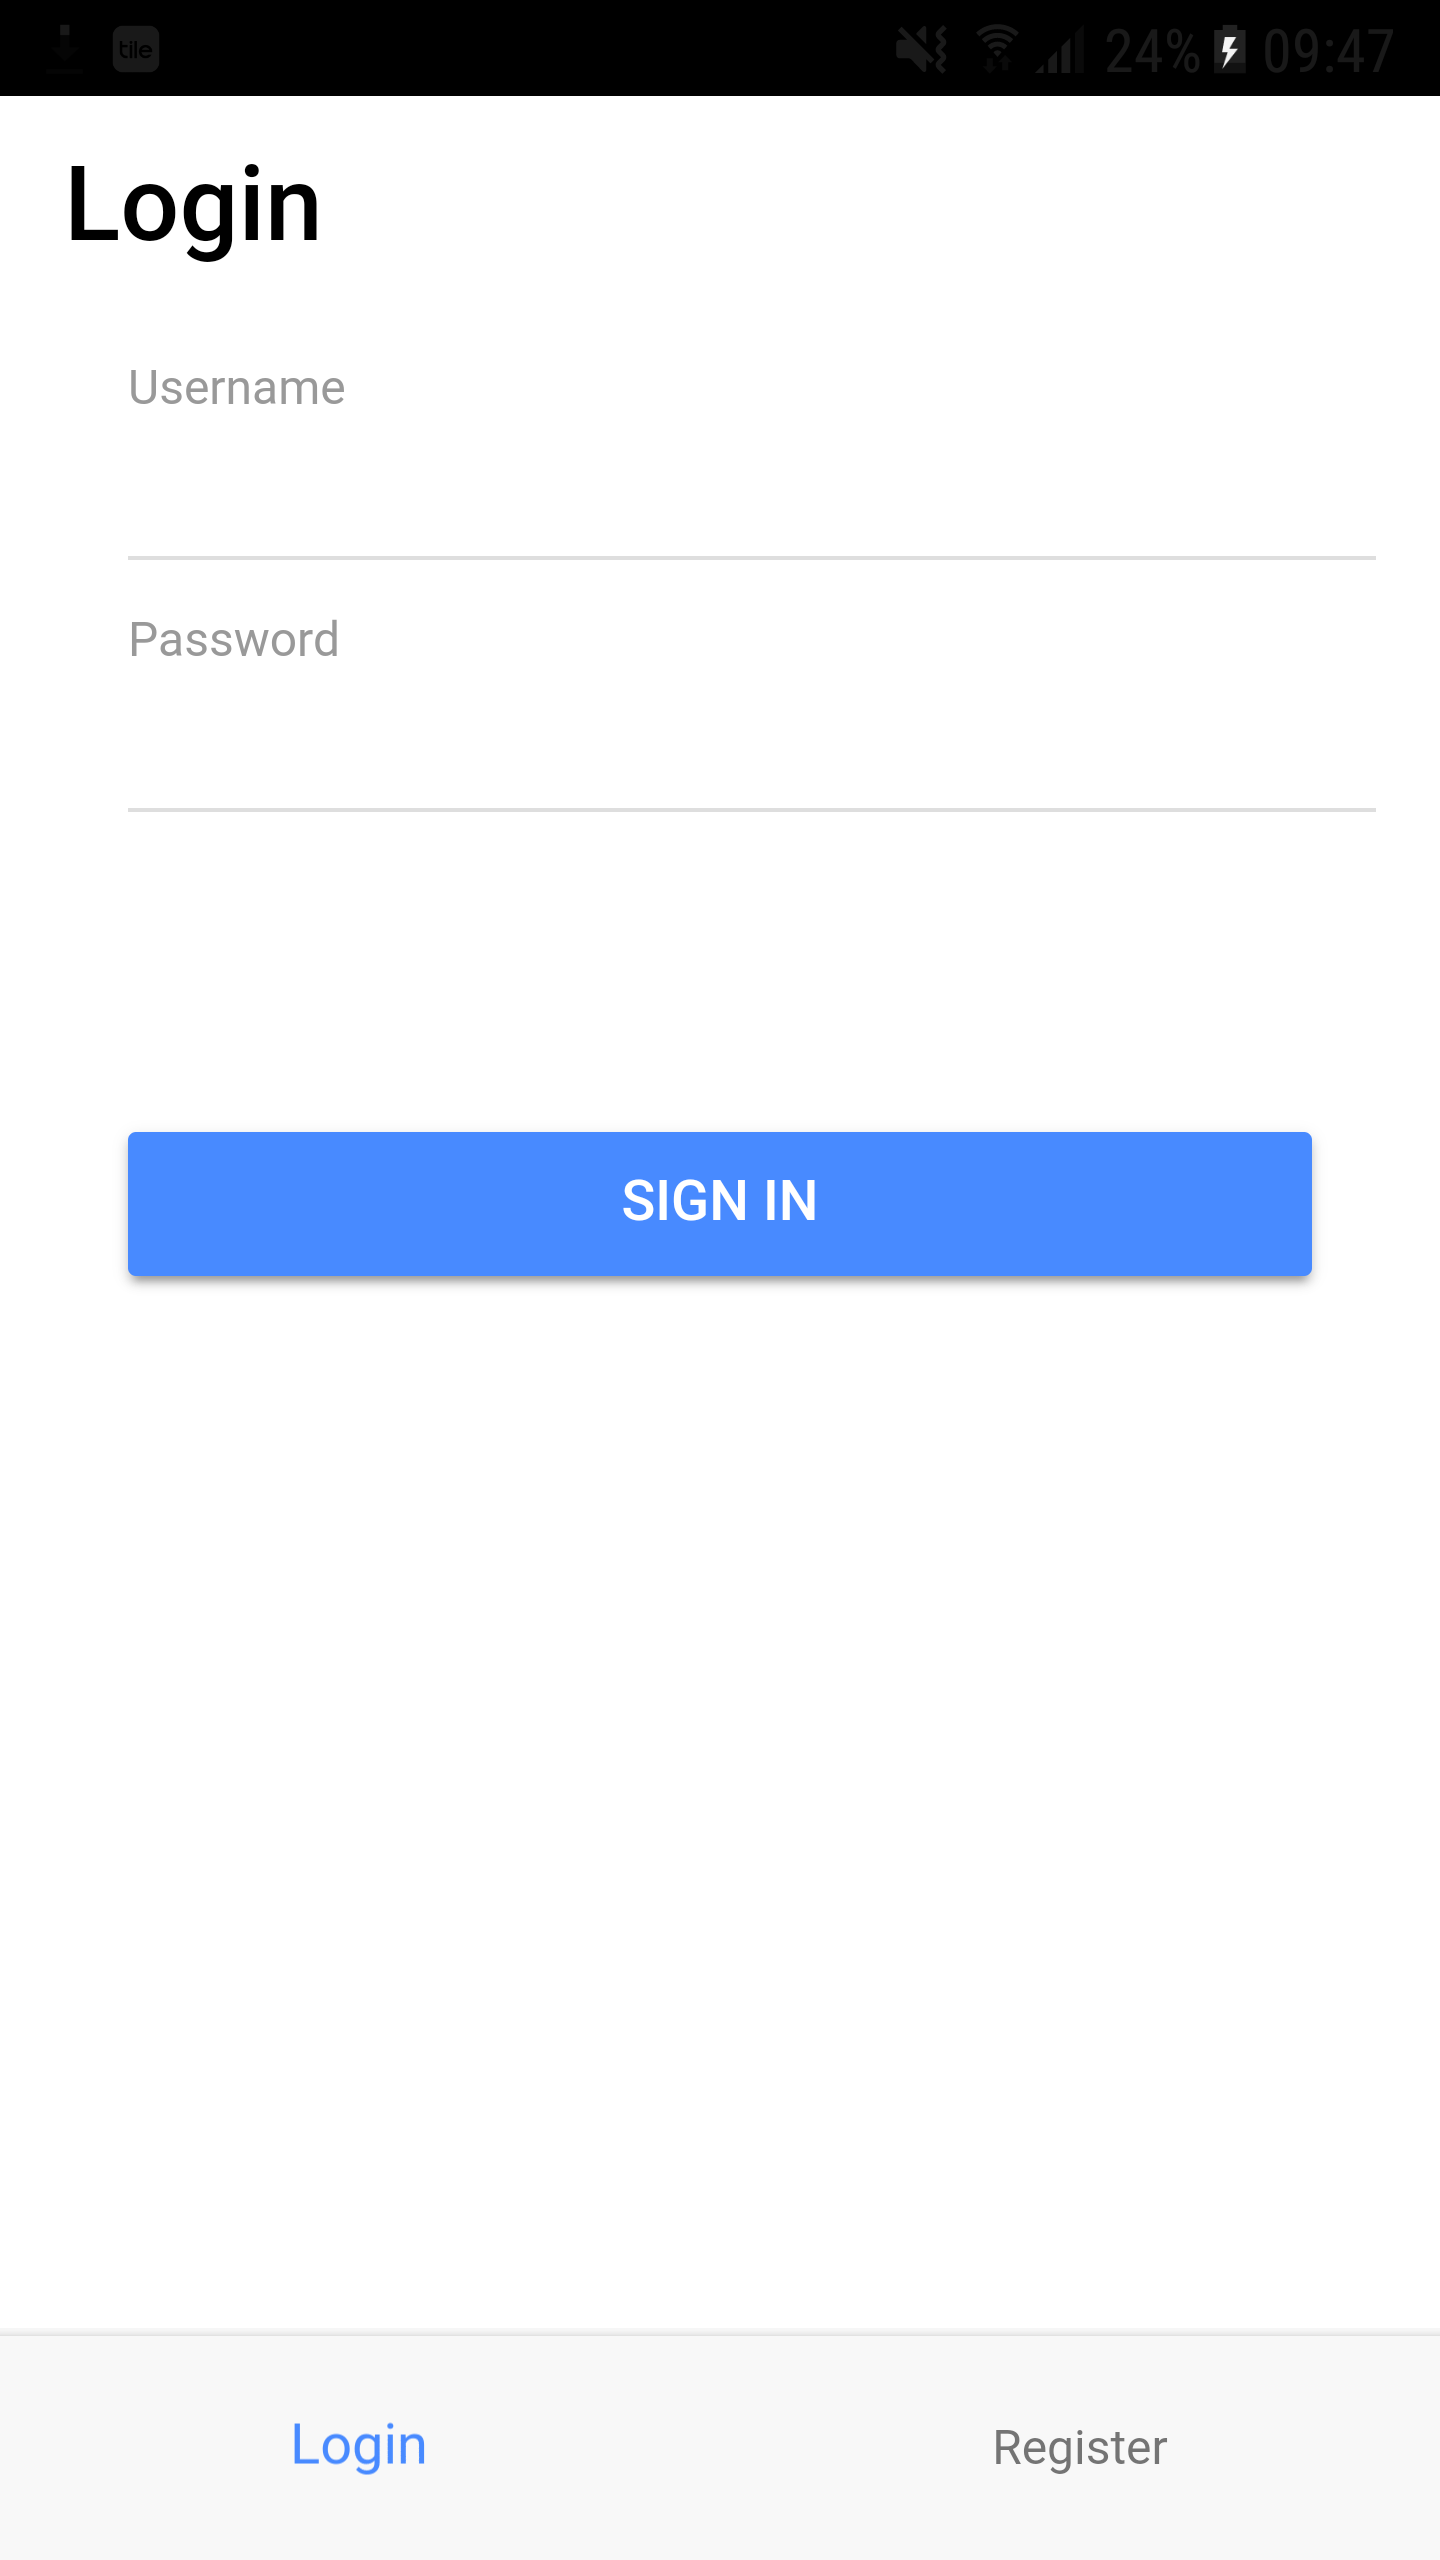
\includegraphics[width=0.4\textwidth]{images/login_page}}
	\quad
	\subfloat[Ekran rejestracji.]{\label{odnosnik}
		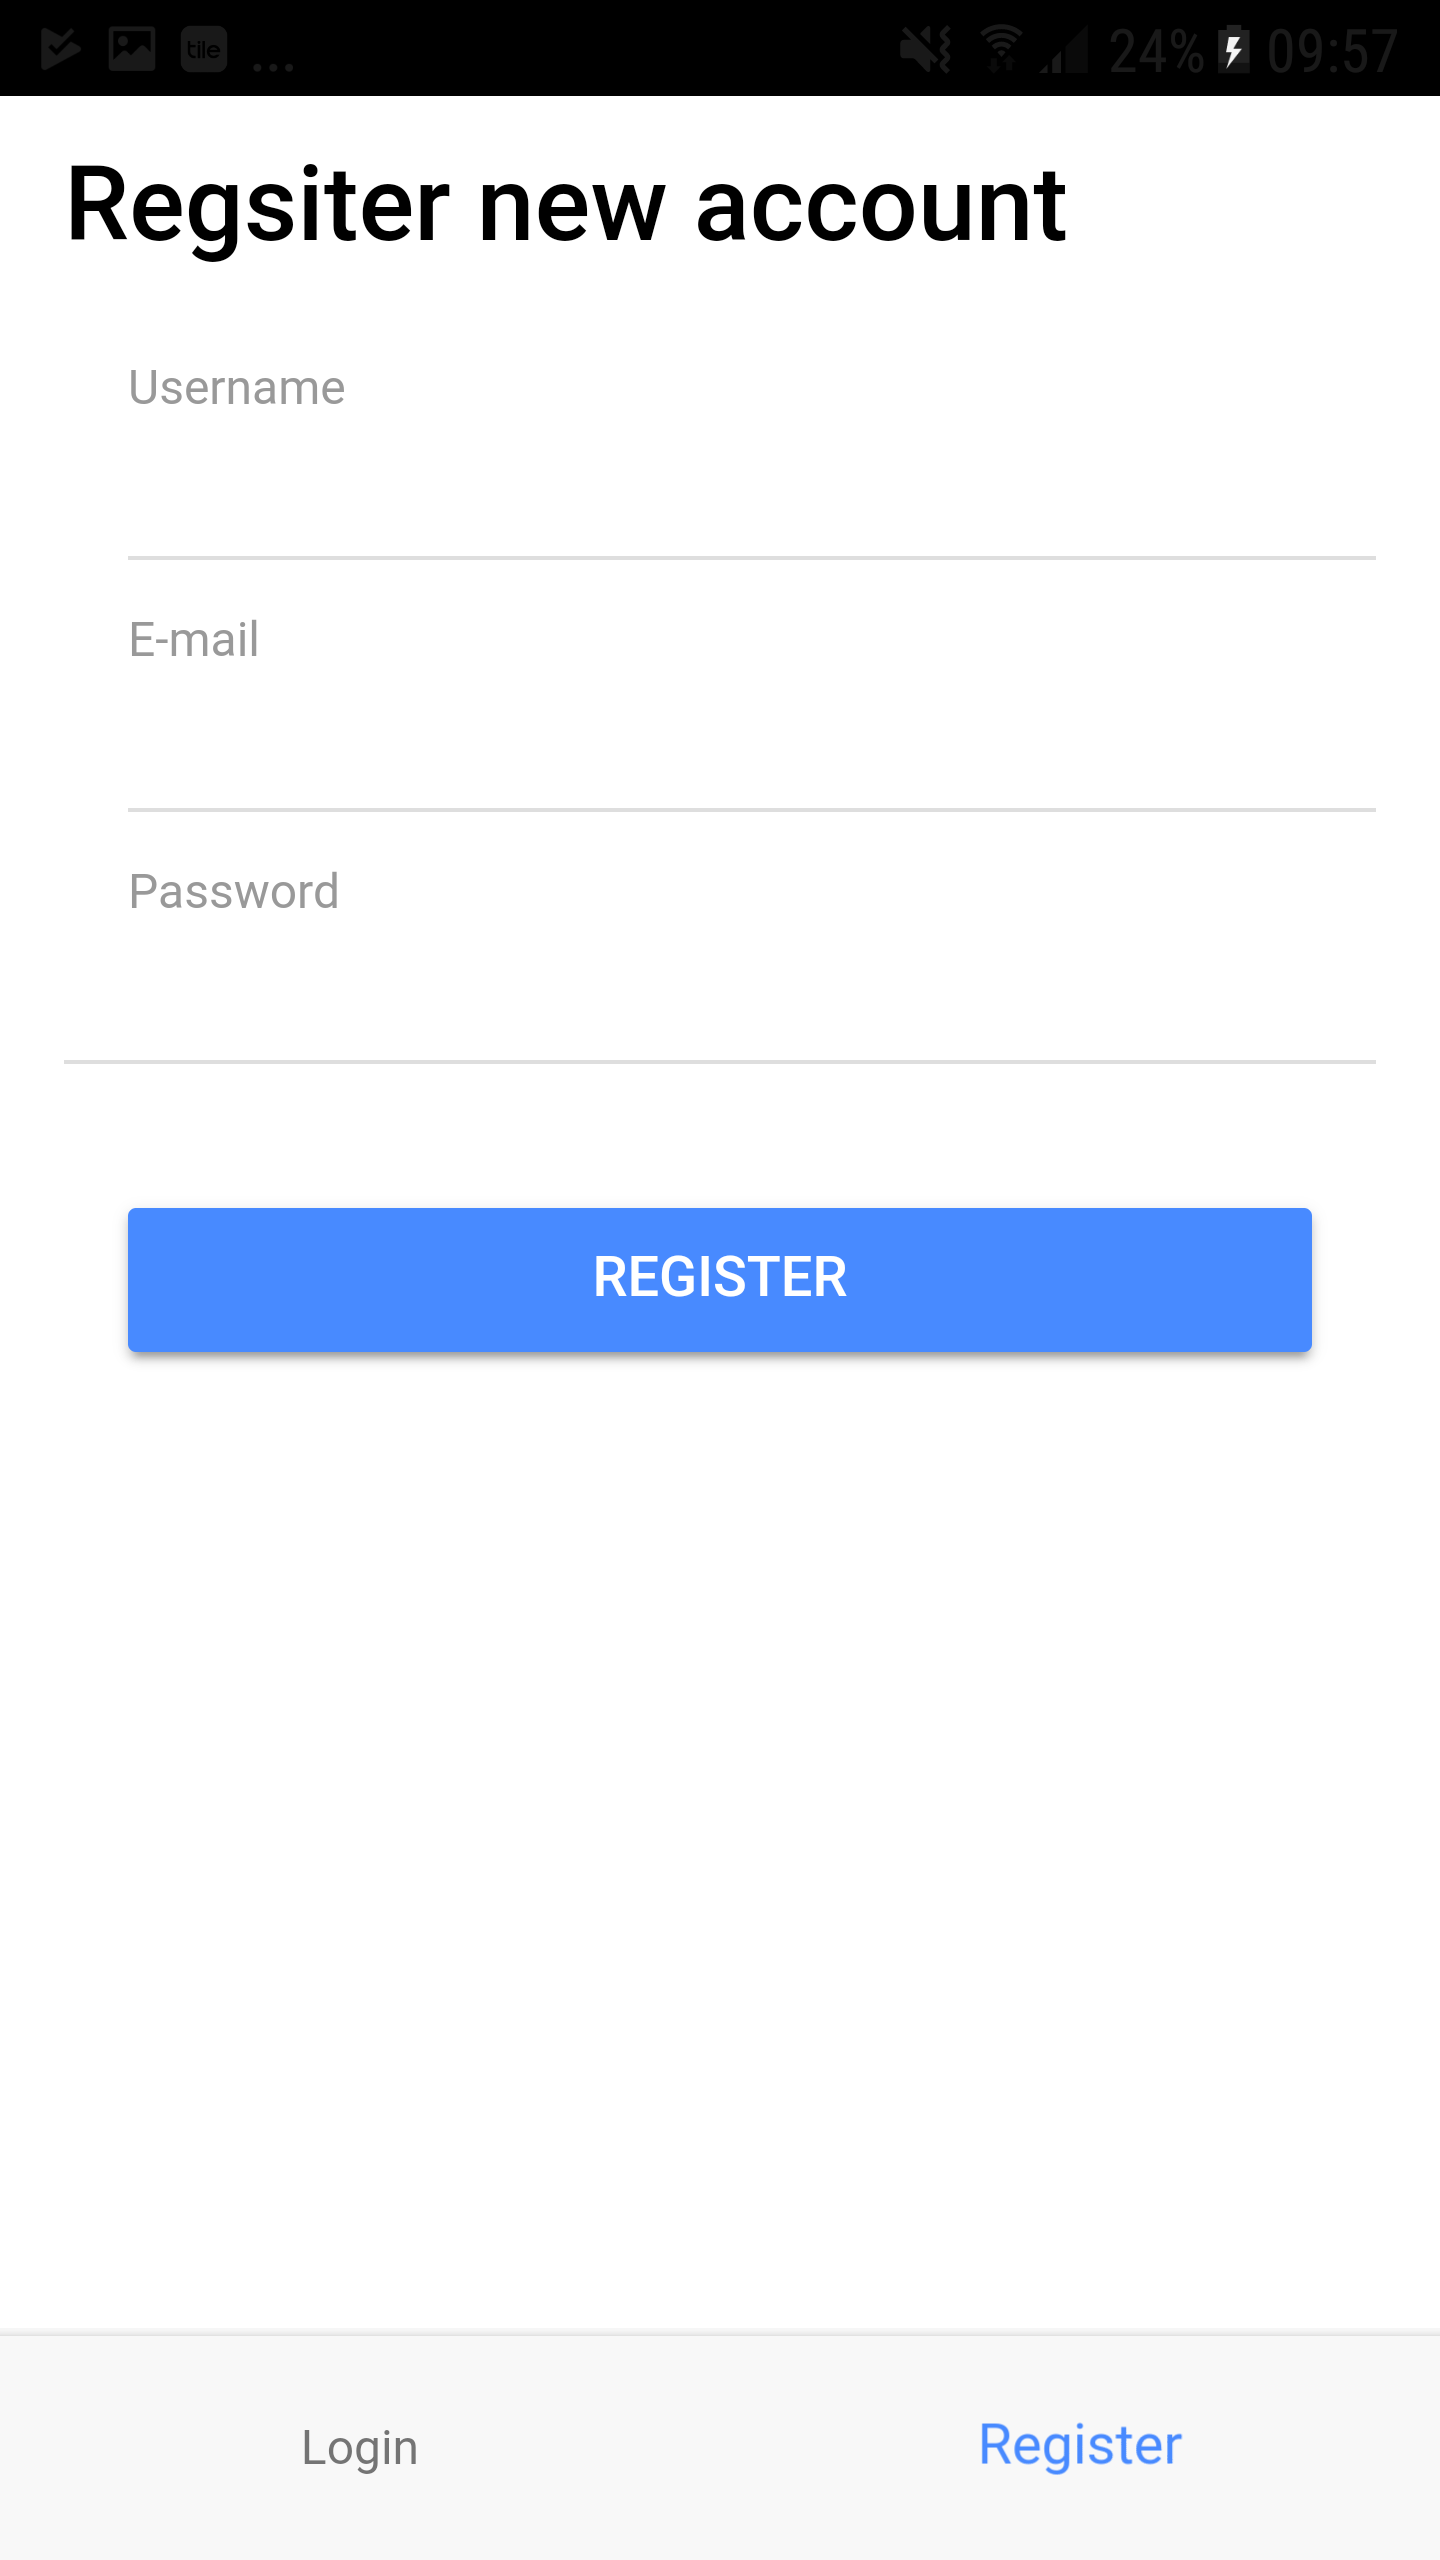
\includegraphics[width=0.4\textwidth]{images/register_page}}
	\caption{Ekrany logowania i rejestracji}
	\label{fig:registerpage}
\end{figure}

W przypadku gdy użytkownik nie posiada konta, zalecane jest skorzystanie z zakładki "Rejestracja". Umożliwia ona wpisanie podstawowych informacji niezbędnych do założenia konta. Zostały nałożone również restrykcje dotyczące polityki bezpieczeństwa konta. W związku z tym podczas rejestracji użytkownik jest proszony o:
\begin{itemize}[noitemsep]
	\item podanie adresu e-mail,
	\item podanie unikalnej nazwy użytkownika,
	\item ustawienie hasła zawierającego co najmniej trzy znaki.
\end{itemize} 
}
\newpage
\section{Scenariusz użycia}{

Pomyślna rejestracja oraz zalogowanie użytkownika przenoszą go do ekranu głównego aplikacji. Pierwszy widok zawiera instrukcje zachęcające do zrobienia nowego zdjęcia lub wybrania go z galerii. Ponadto na ekranie dostępne są dodatkowe zakładki - "History", "Report" oraz "Contact". Użytkownik ma możliwość wylogowania się dzięki przyciskowi "Logout" znajdującemu się w prawym górnym rogu ekranu. Pierwszy ekran umożliwia przesłanie zdjęcia do serwera aplikacji w celu dalszego przetwarzania. Aby zrobić zdjęcie, należy wybrać przycisk "TAKE PHOTO", który uruchomi kamerę. Aplikacja będzie oczekiwała do momentu przekazania zdjęcia z aparatu. W przypadku wybrania przycisku "SELECT FROM GALLERY", aplikacja uruchomi systemowy eksplorator zdjęć. Wybór jednego z nich będzie równoznaczny dla aplikacji ze zrobieniem zdjęcia z aparatu. ProductScanner po wybraniu obrazu wyświetli go na ekranie głównym oraz udostępni przyciski "Send" oraz "Remove". Wybranie przycisku "Send" prześle zdjęcie na serwer. W przypadku przycisku "Remove" zdjęcie zostanie usunięte. Opisywany ekran został przedstawiony na rysunku \ref{fig:uploadView}. Użytkownik z ekranu głównego aplikacji ma dostęp do zakładki kontakt. Zostały w niej zawarte informacje o autorze aplikacji.

	
\begin{figure}[h]
	\centering
	\subfloat[Główny widok aplikacji.]{\label{odnosnik}
		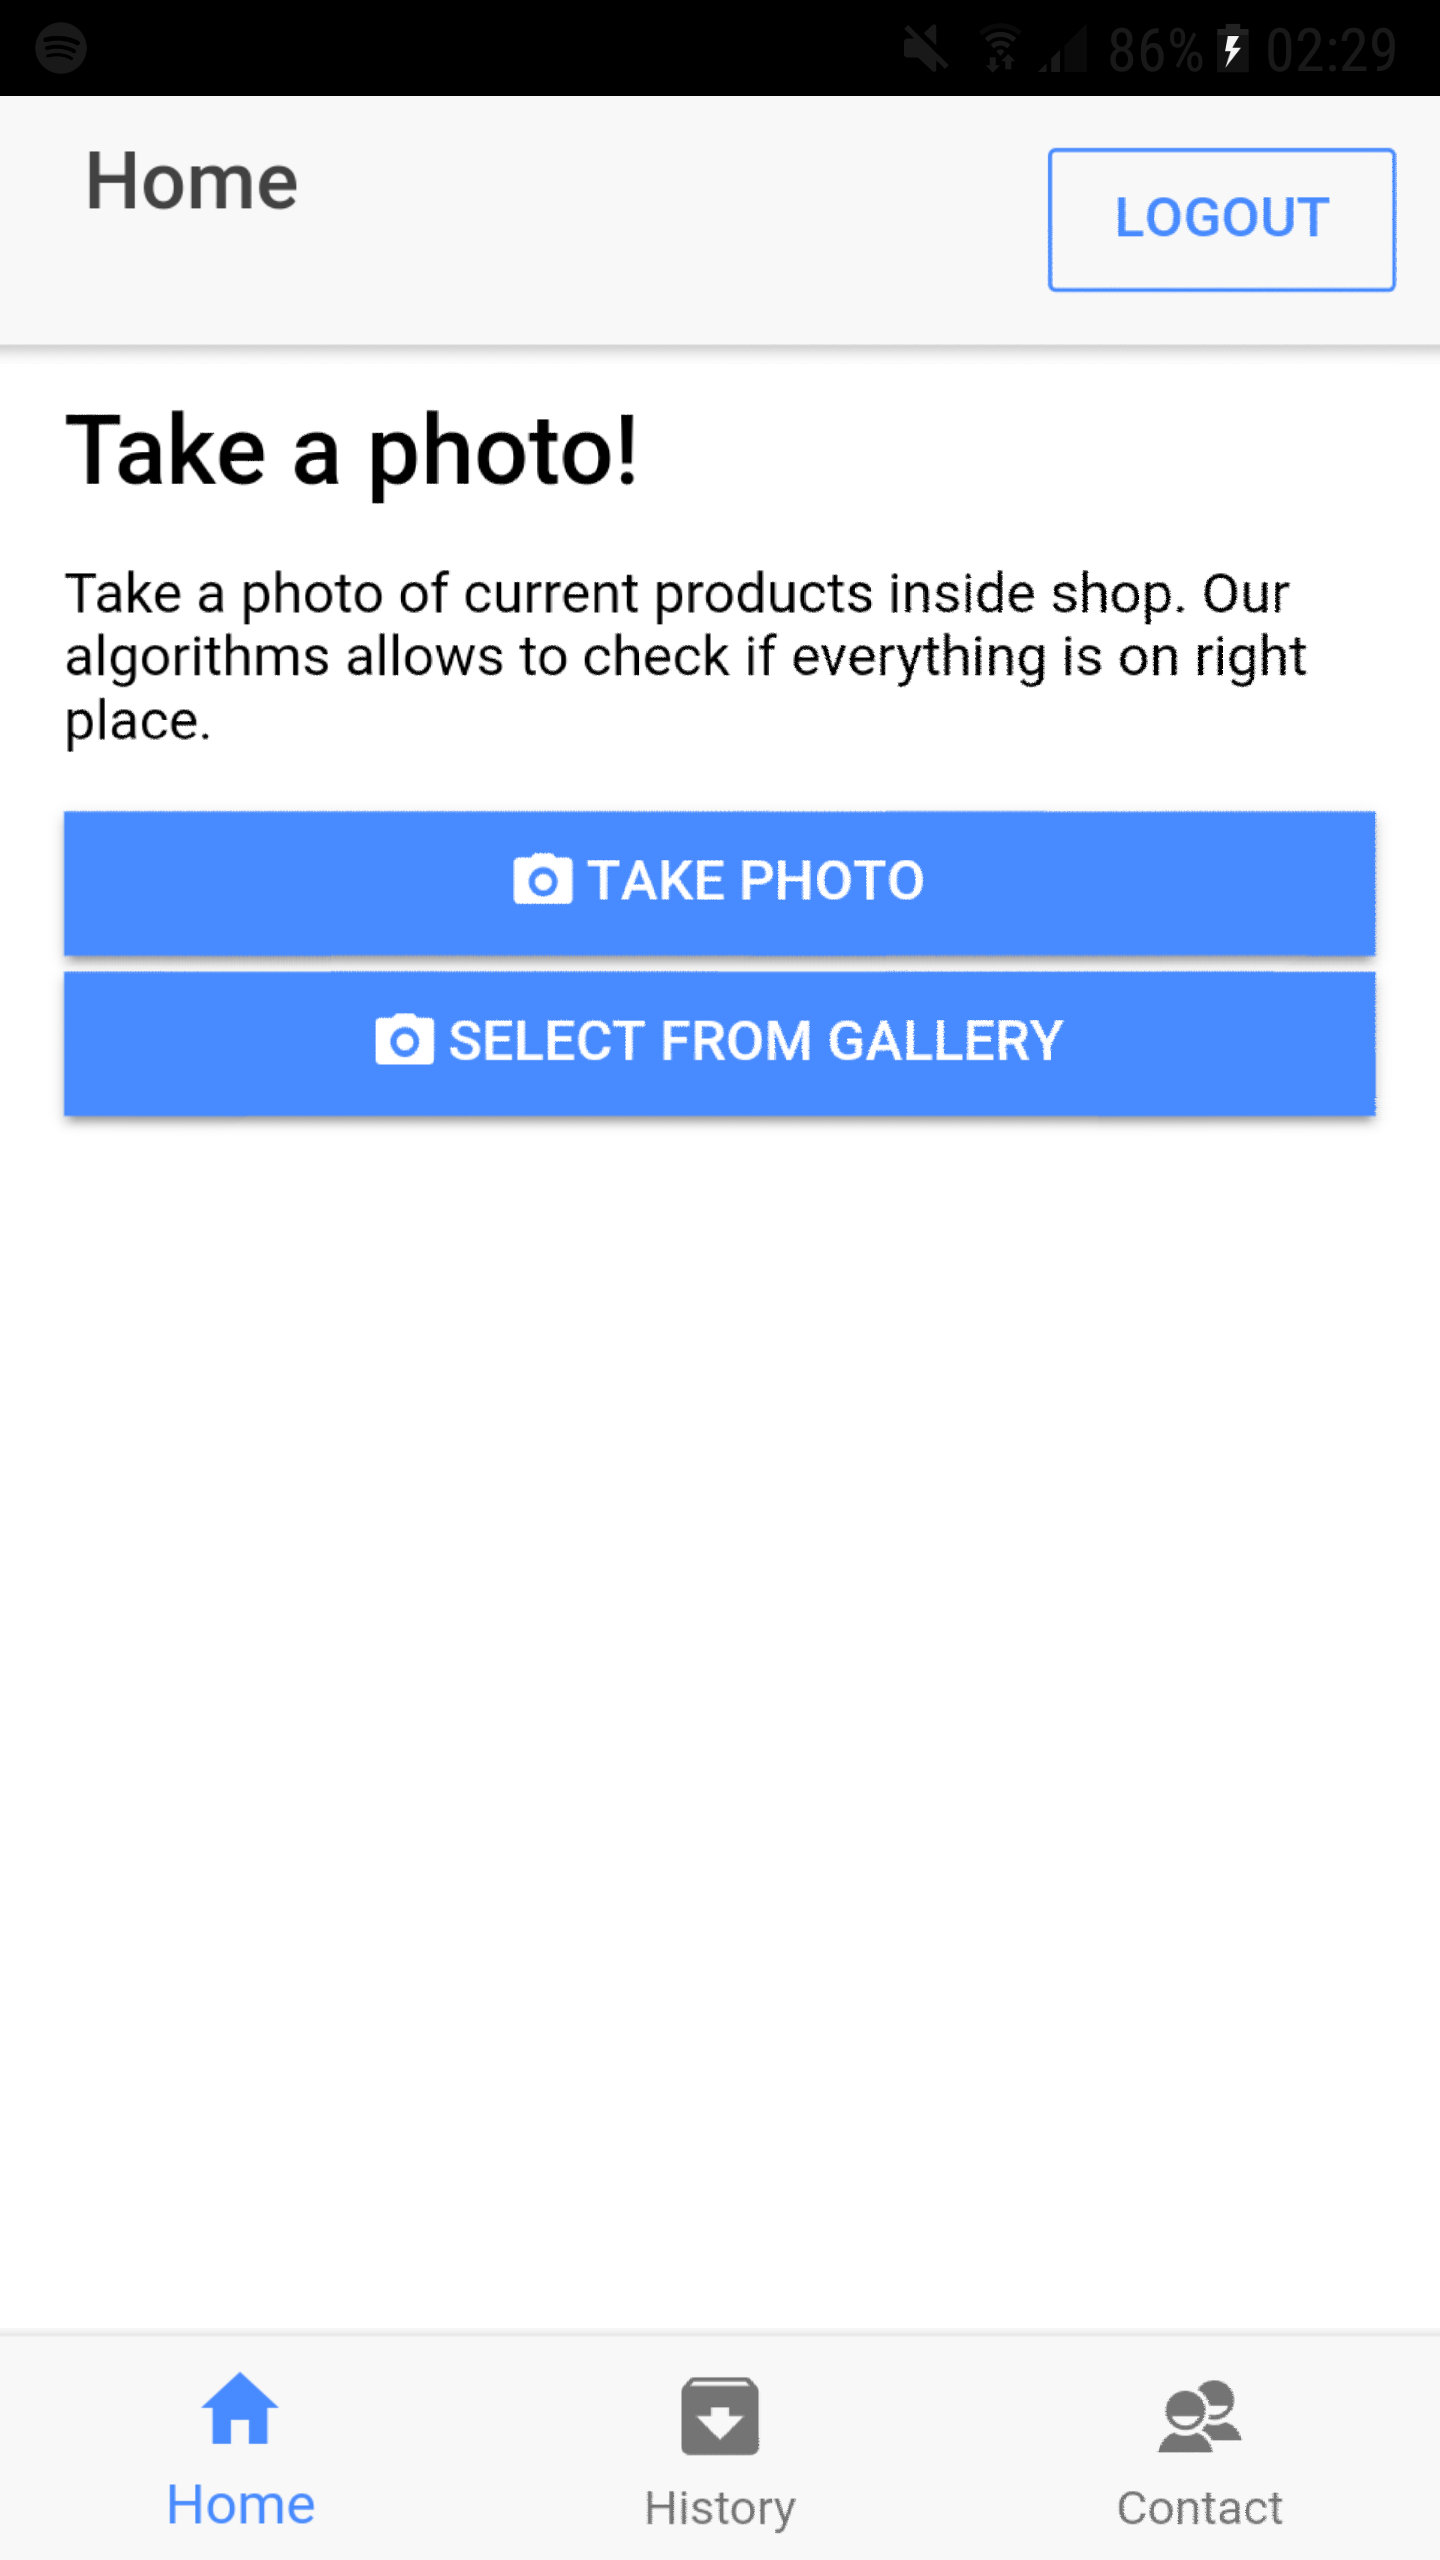
\includegraphics[width=0.4\textwidth]{images/home_page}}
	\quad
	\subfloat[Widok wysłania zdjęcia.]{\label{odnosnik}
		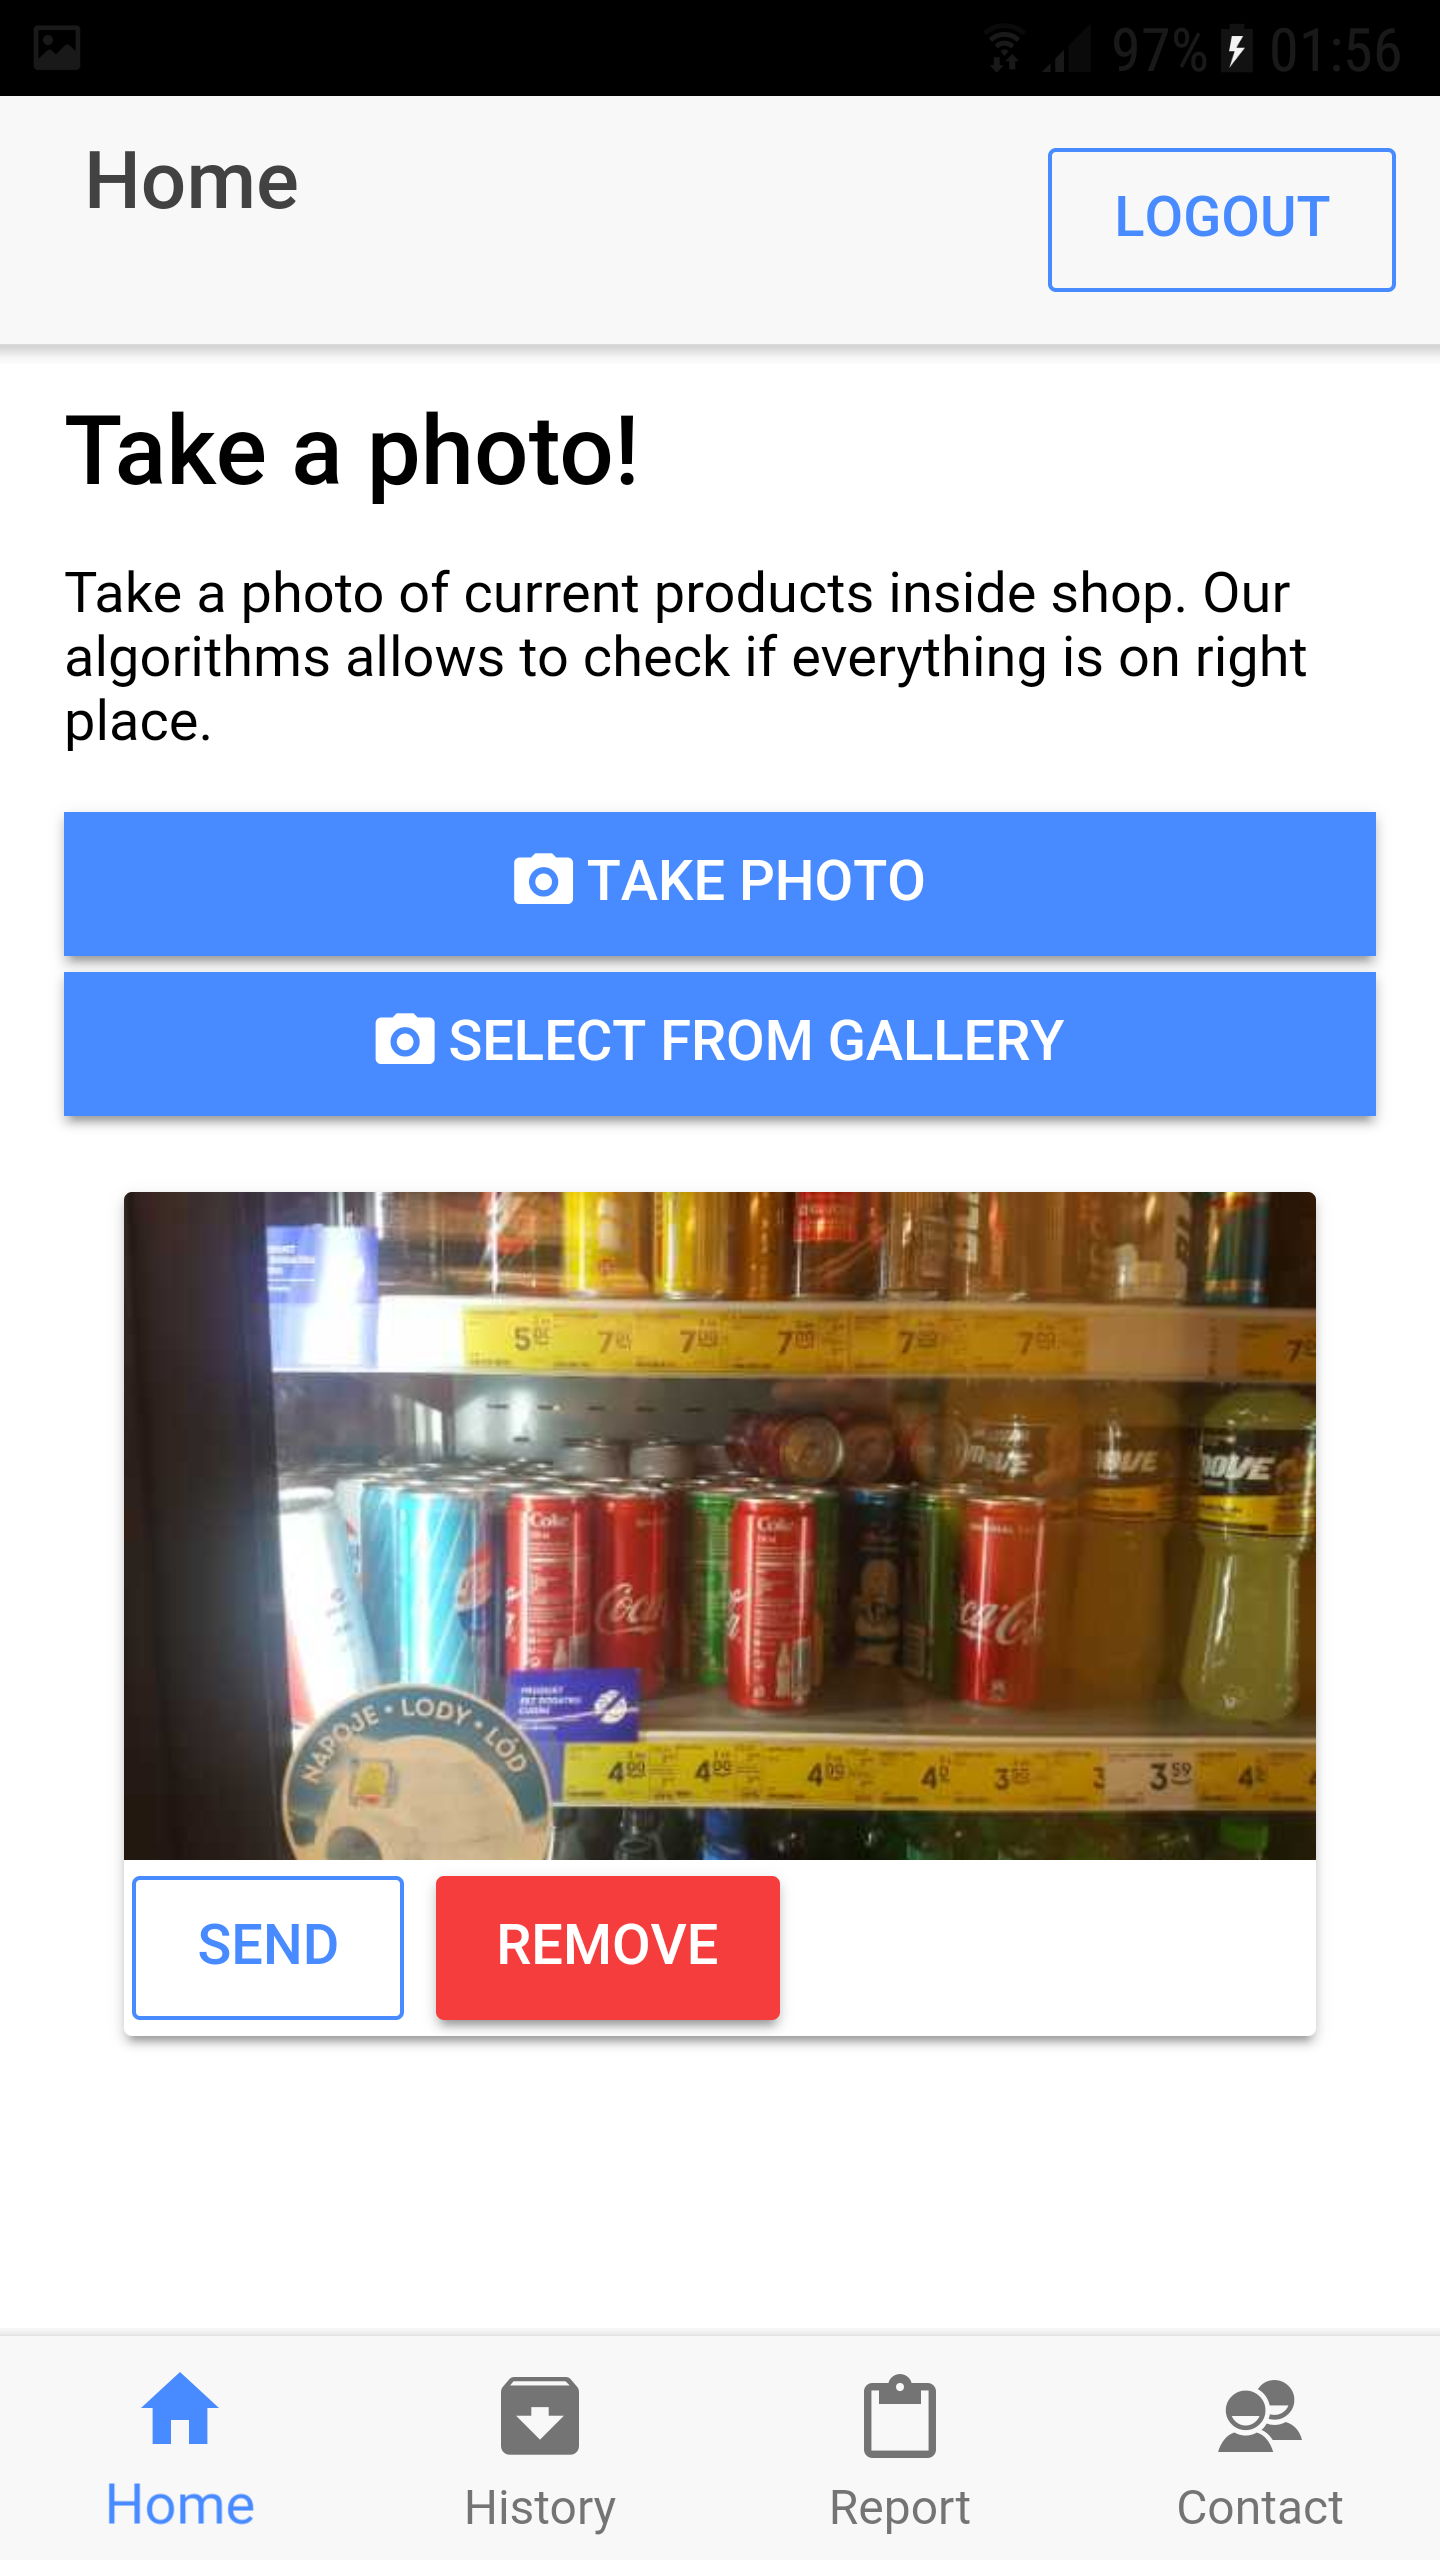
\includegraphics[width=0.4\textwidth]{images/upload_page}}
	\caption{Ekran domowy oraz wysłania zdjęcia.}
	\label{fig:uploadView}
\end{figure}

Użytkownik w celu poddania zdjęcia analizie może wybrać je z galerii lub wykonać je przy użyciu aparatu z ekranu głównego. Udostępnienie zdjęcia na serwer spowoduje uruchomienie algorytmów detekcji przedmiotów oraz przetwarzania ontologii. W momencie oczekiwania na dokonanie obliczeń użytkownik czeka na odpowiedź serwera na ekranie ładowania. Po zakończeniu przetwarzania danych ekran wyświetli okno szczegółów analizy. Dzięki niemu użytkownik może poznać wyniki klasyfikacji przedmiotów oraz przetwarzania reguł semantycznych. Ekran został podzielony na trzy sekcje - zdjęcie (Image), typy (Types) oraz wartości (Values). Zakładka zdjęcia (Image) zawiera aktualnie przetworzone zdjęcie wraz z zaznaczeniem przedmiotów na nim oraz ich pozycje. Wynik klasyfikacji przedmiotów znajdujący się na półkach sklepowych został przedstawiony na rysunku \ref{fig:classificationImages}. 
\begin{figure}[h]
	\centering
	\subfloat[Klasyfikacja przedmiotów na półce sklepowej.]{\label{odnosnik}
		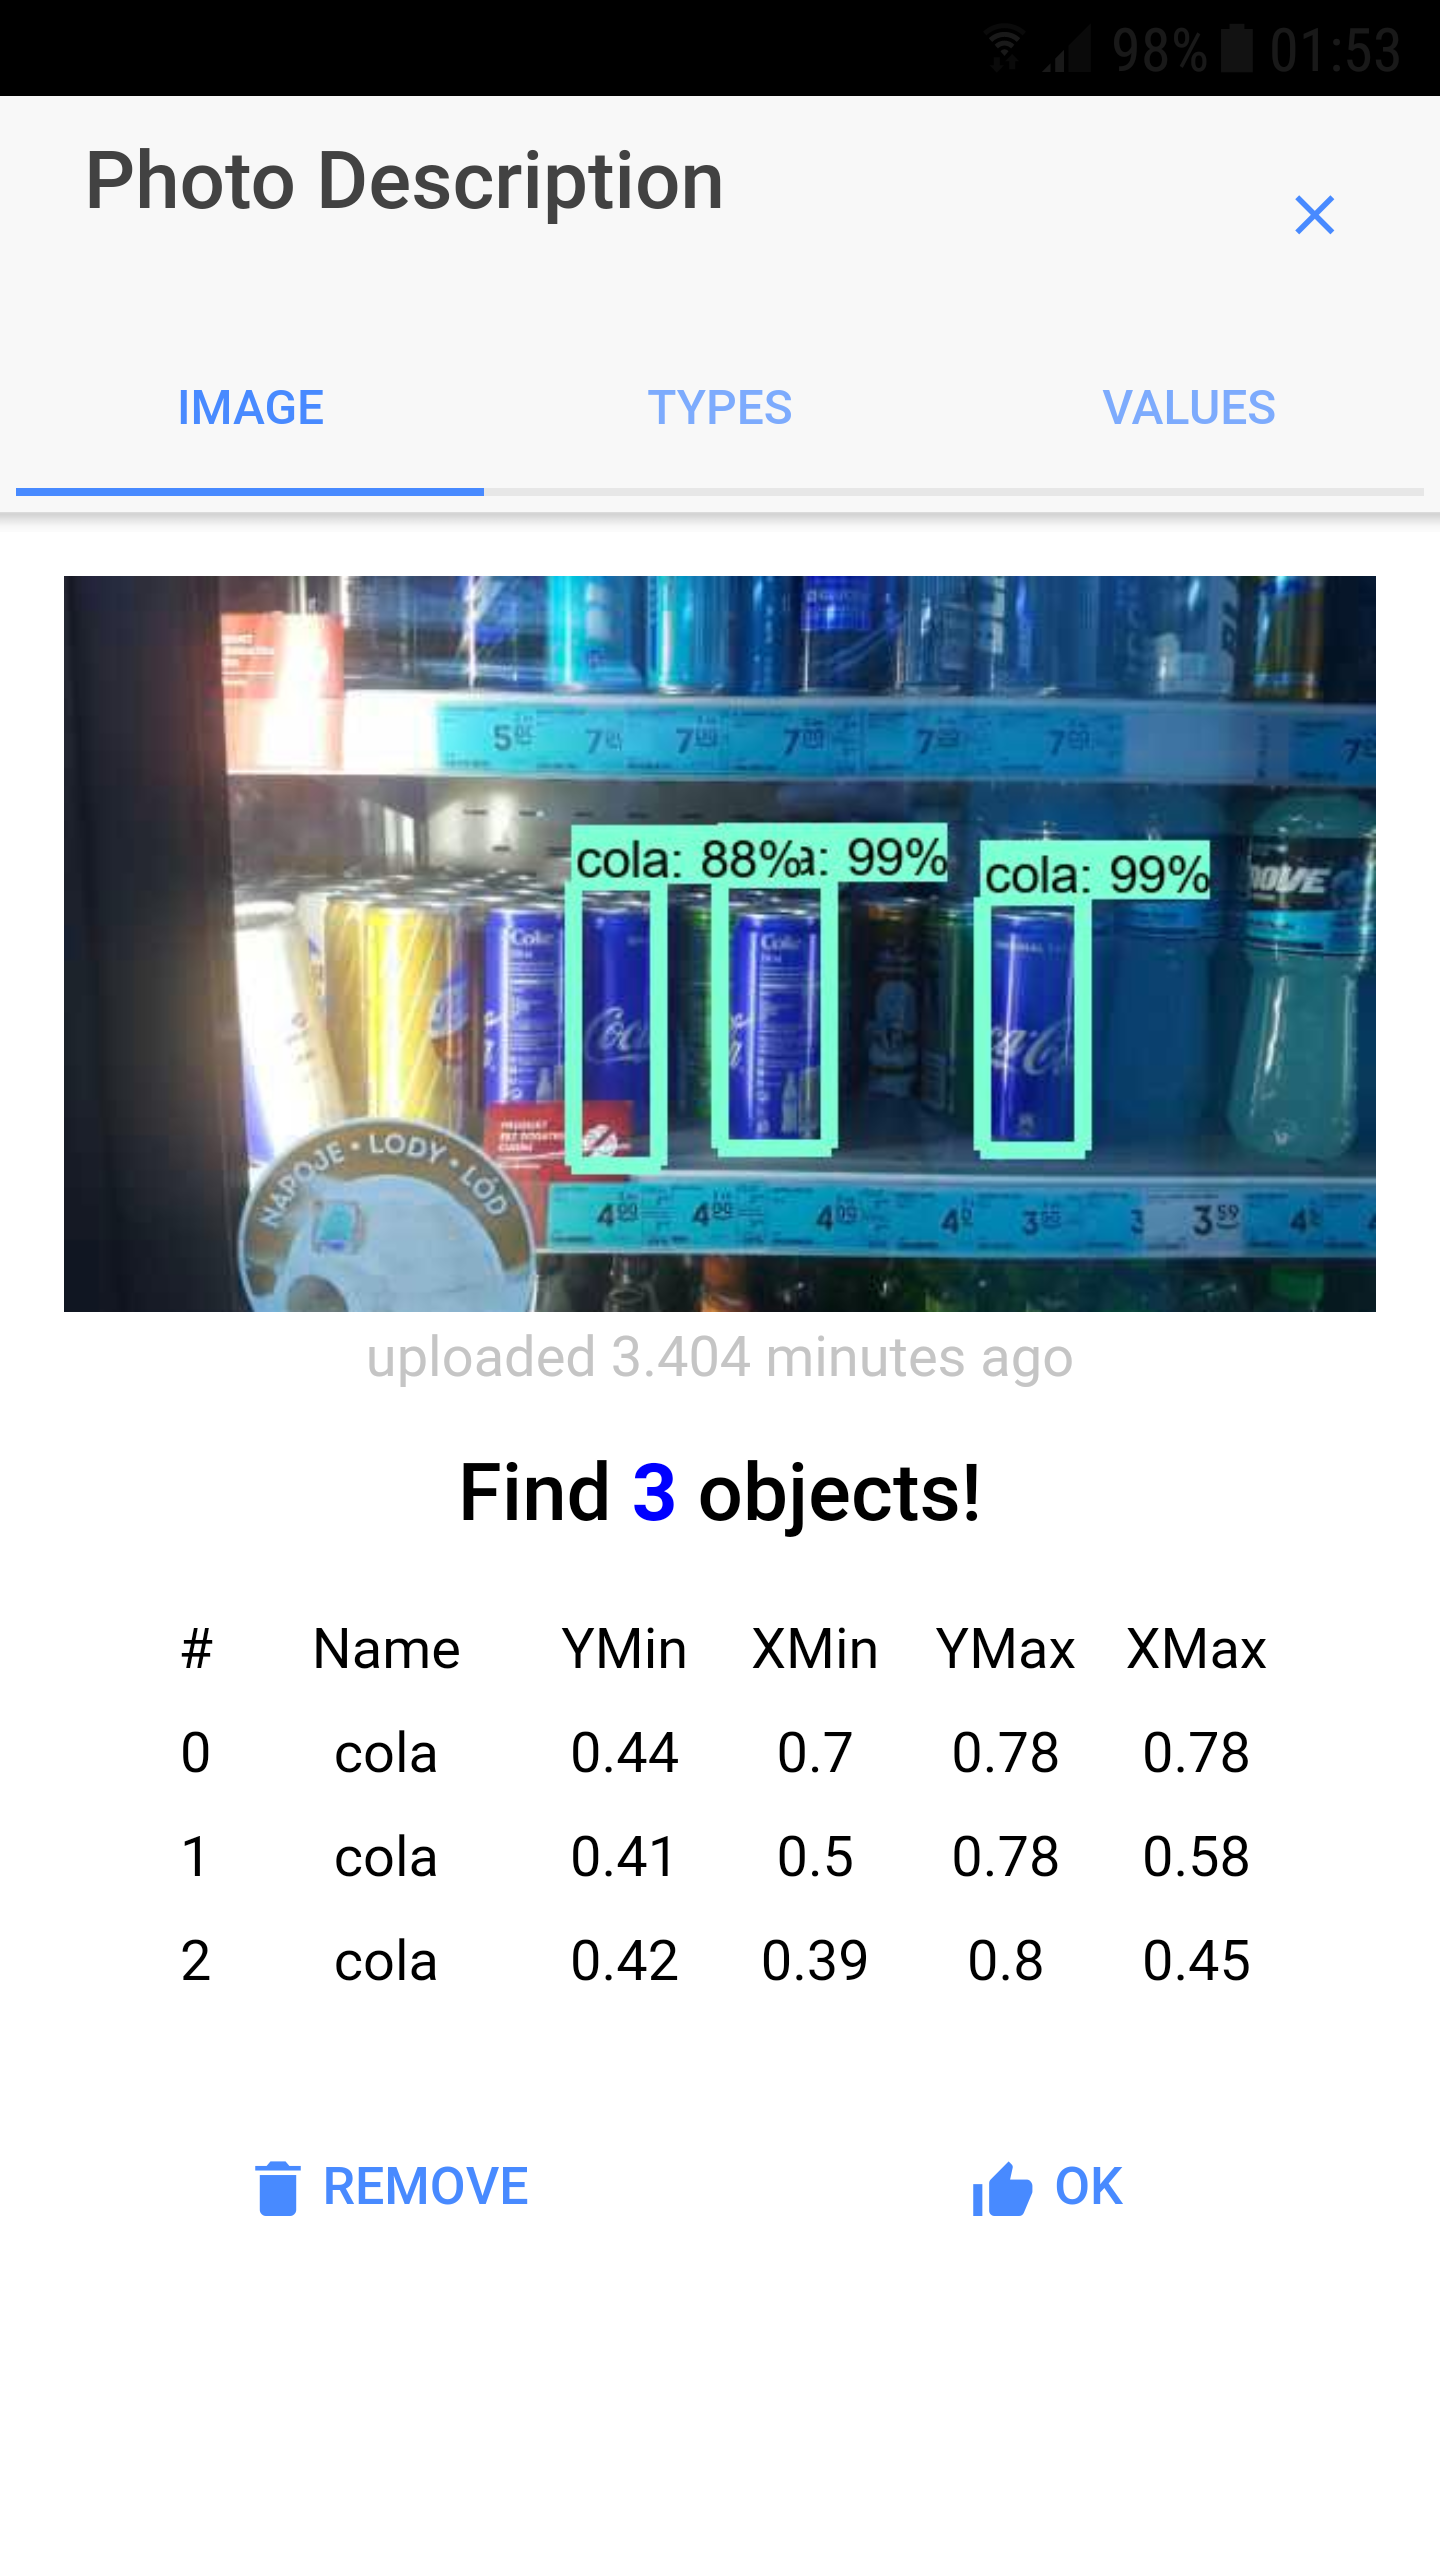
\includegraphics[width=0.4\textwidth]{images/details}}
	\quad
	\subfloat[Klasyfikacja przedmiotów na półce sklepowej.]{\label{odnosnik}
		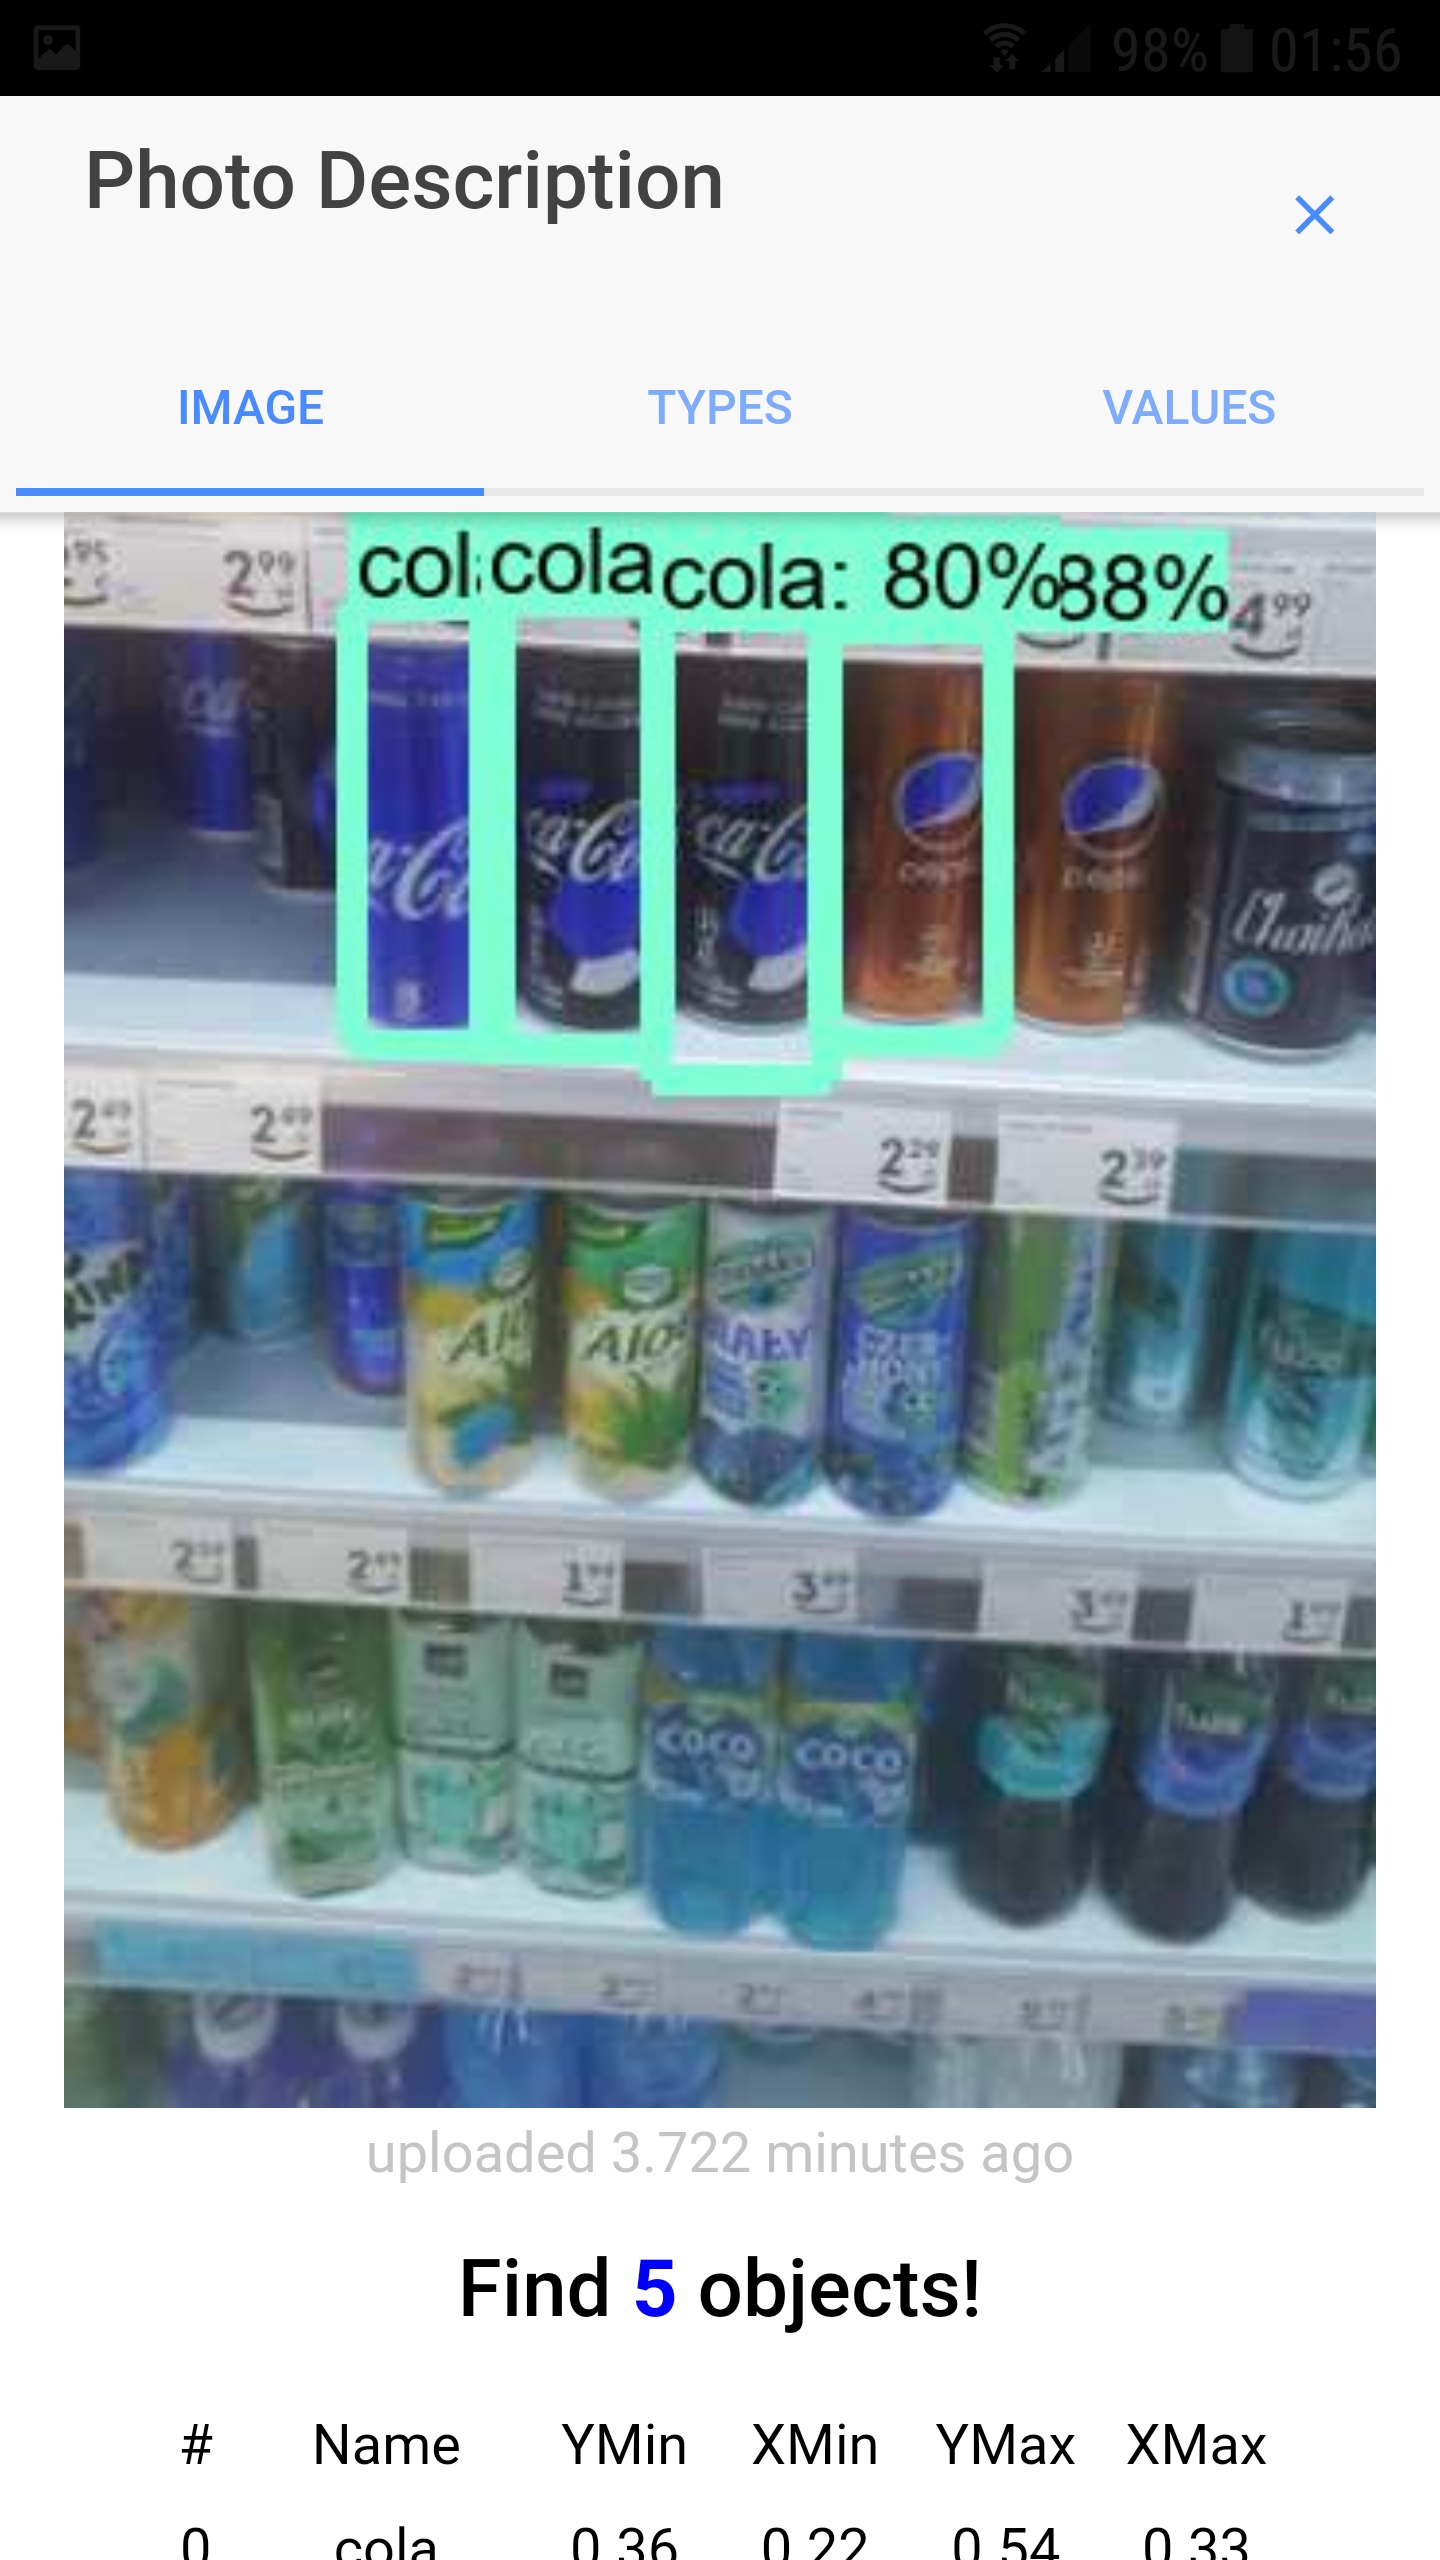
\includegraphics[width=0.4\textwidth]{images/details2}}
	\caption{Ekran szczegółów analizowanego zdjęcia - podzakładka klasyfikacji przedmiotów.}
	\label{fig:classificationImages}
	
\end{figure}

Przejście do zakładki typów (Types) spowoduje wyświetlenie zbiorów typów sklasyfikowanych przedmiotów dla danego zdjęcia. Dzięki temu użytkownik może wywnioskować, że wykryty napój jest gazowany oraz ma barwę. Z informacji można wywnioskować, czy dane indywiduum jest typu "Invalid". Będzie to oznaczało niepoprawne ułożenie produktu względem reszty przedmiotów. Zakładka "Types" z uzyskanymi typami produktów została przedstawiona na rysunku \ref{fig:typesView}.

\begin{figure}[h]
	\centering
	\subfloat[Typy sklasyfikowanych produktów.]{\label{odnosnik}
		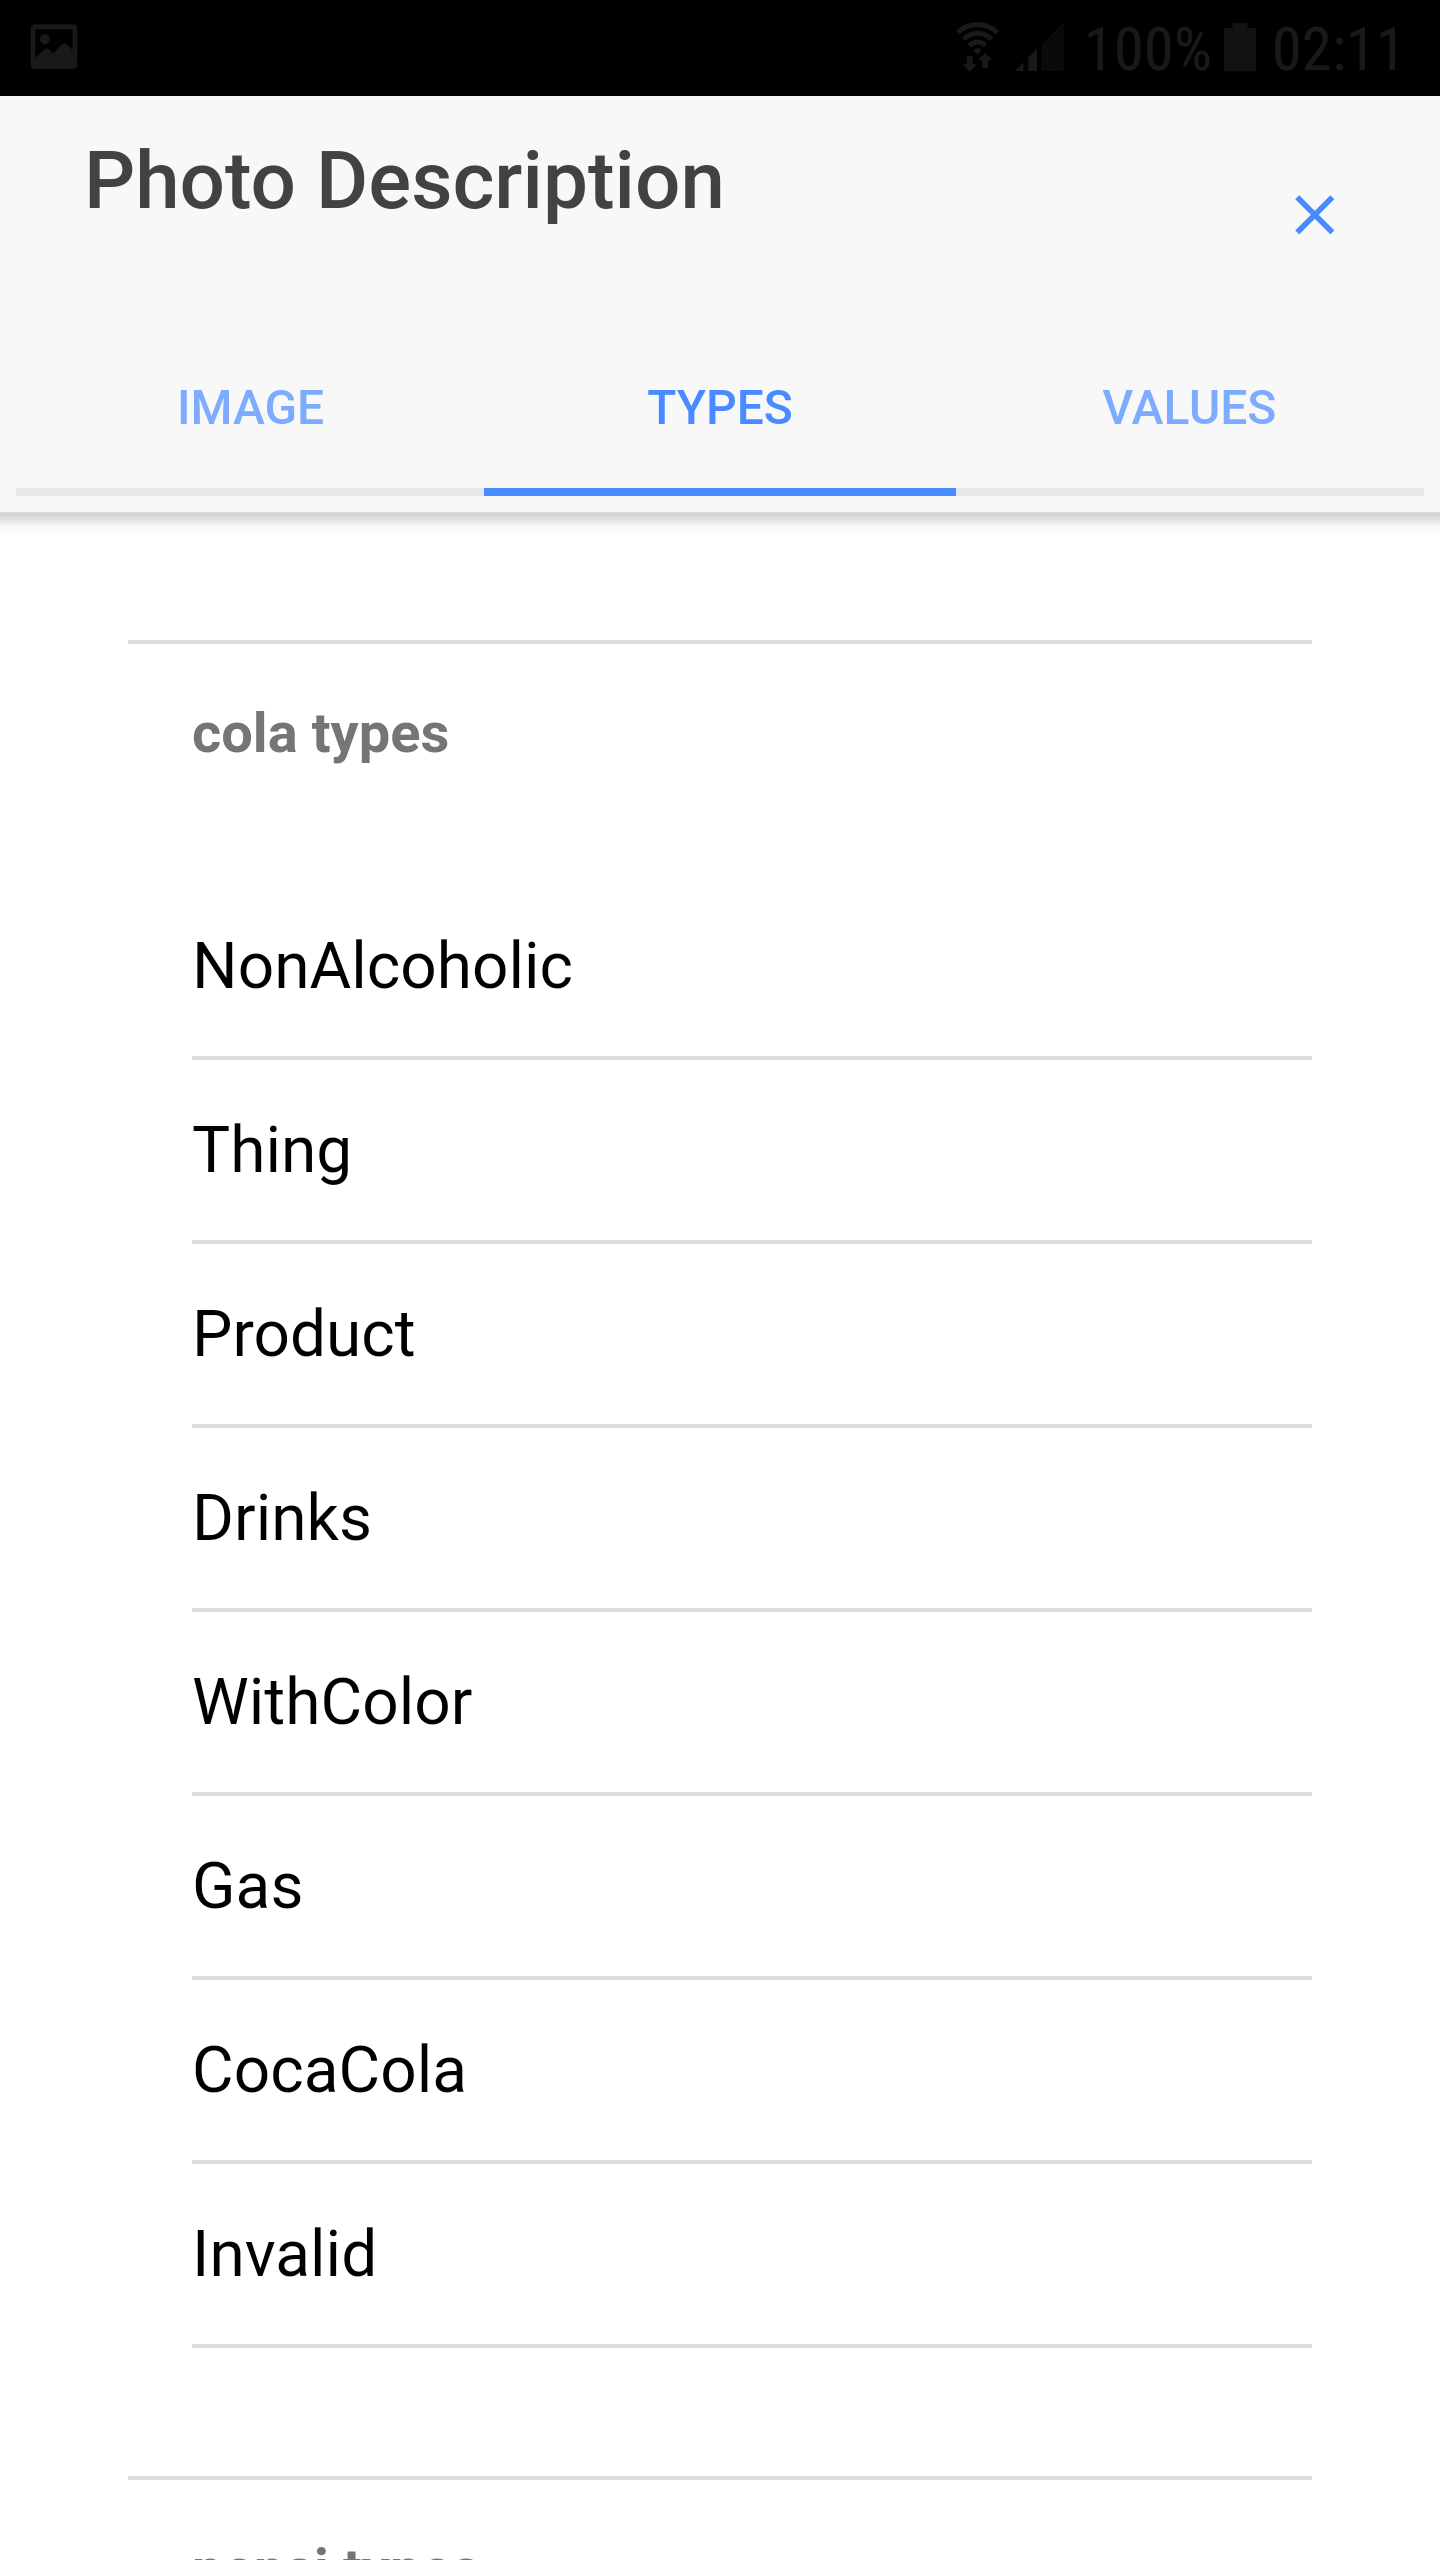
\includegraphics[width=0.4\textwidth]{images/types}}
	\quad
	\subfloat[Typy sklasyfikowanych produktów.]{\label{odnosnik}
		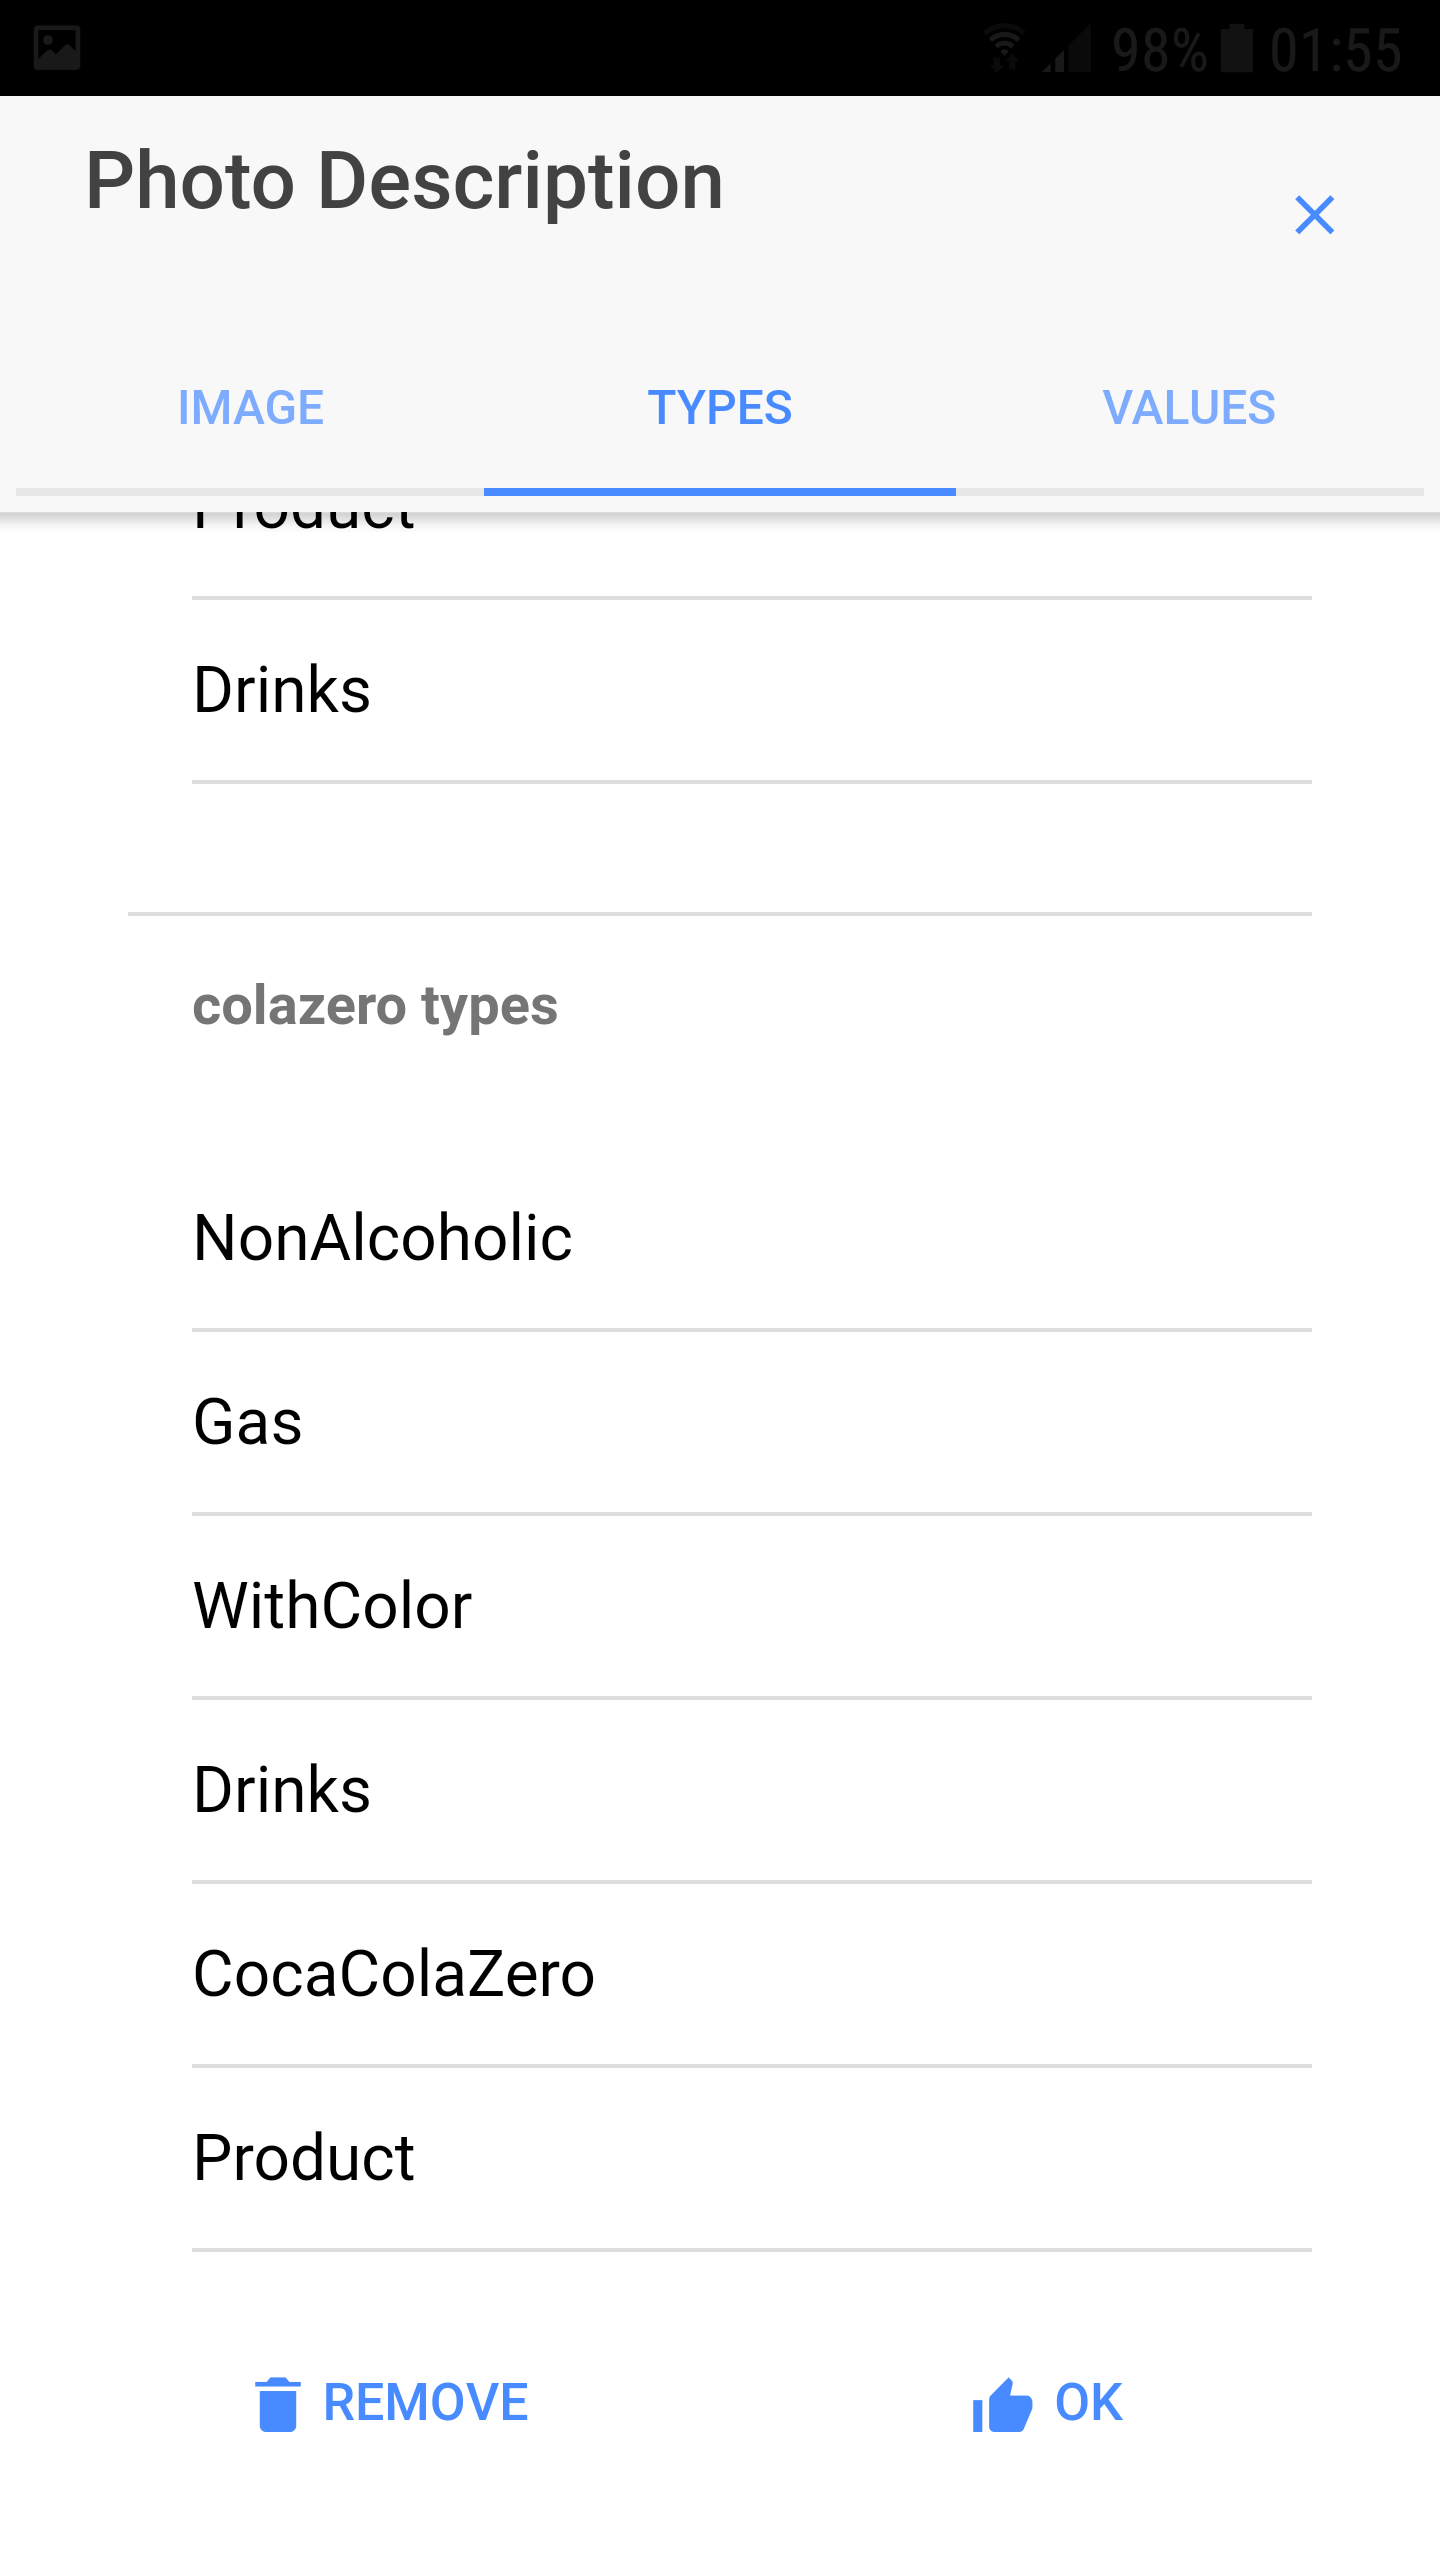
\includegraphics[width=0.4\textwidth]{images/types2}}
	\caption{Ekran szczegółów analizowanego zdjęcia - podzakładka typów produktów.}
	\label{fig:typesView}	
\end{figure}
Przetworzenie ontologii dostarcza informacji o relacjach zachodzących miedzy indywiduami. Dane te użytkownik może znaleźć w zakładce wartości (Values). W przypadku gdy sklasyfikowany przedmiot będzie klasy "Invalid", wówczas w zakładce może znaleźć się informacja opisująca błędne ułożenie.  Aby wyjść z ekranu należy skorzystać z pola x, które znajduje się w prawym górnym rogu ekranu. Wartości wnioskowania ontologii zostały przedstawione na rysunku \ref{fig:details}.
\newpage
\begin{figure}[h]
	\centering
	\subfloat[Relacje pomiędzy indywiduami - wnioski.]{\label{odnosnik}
		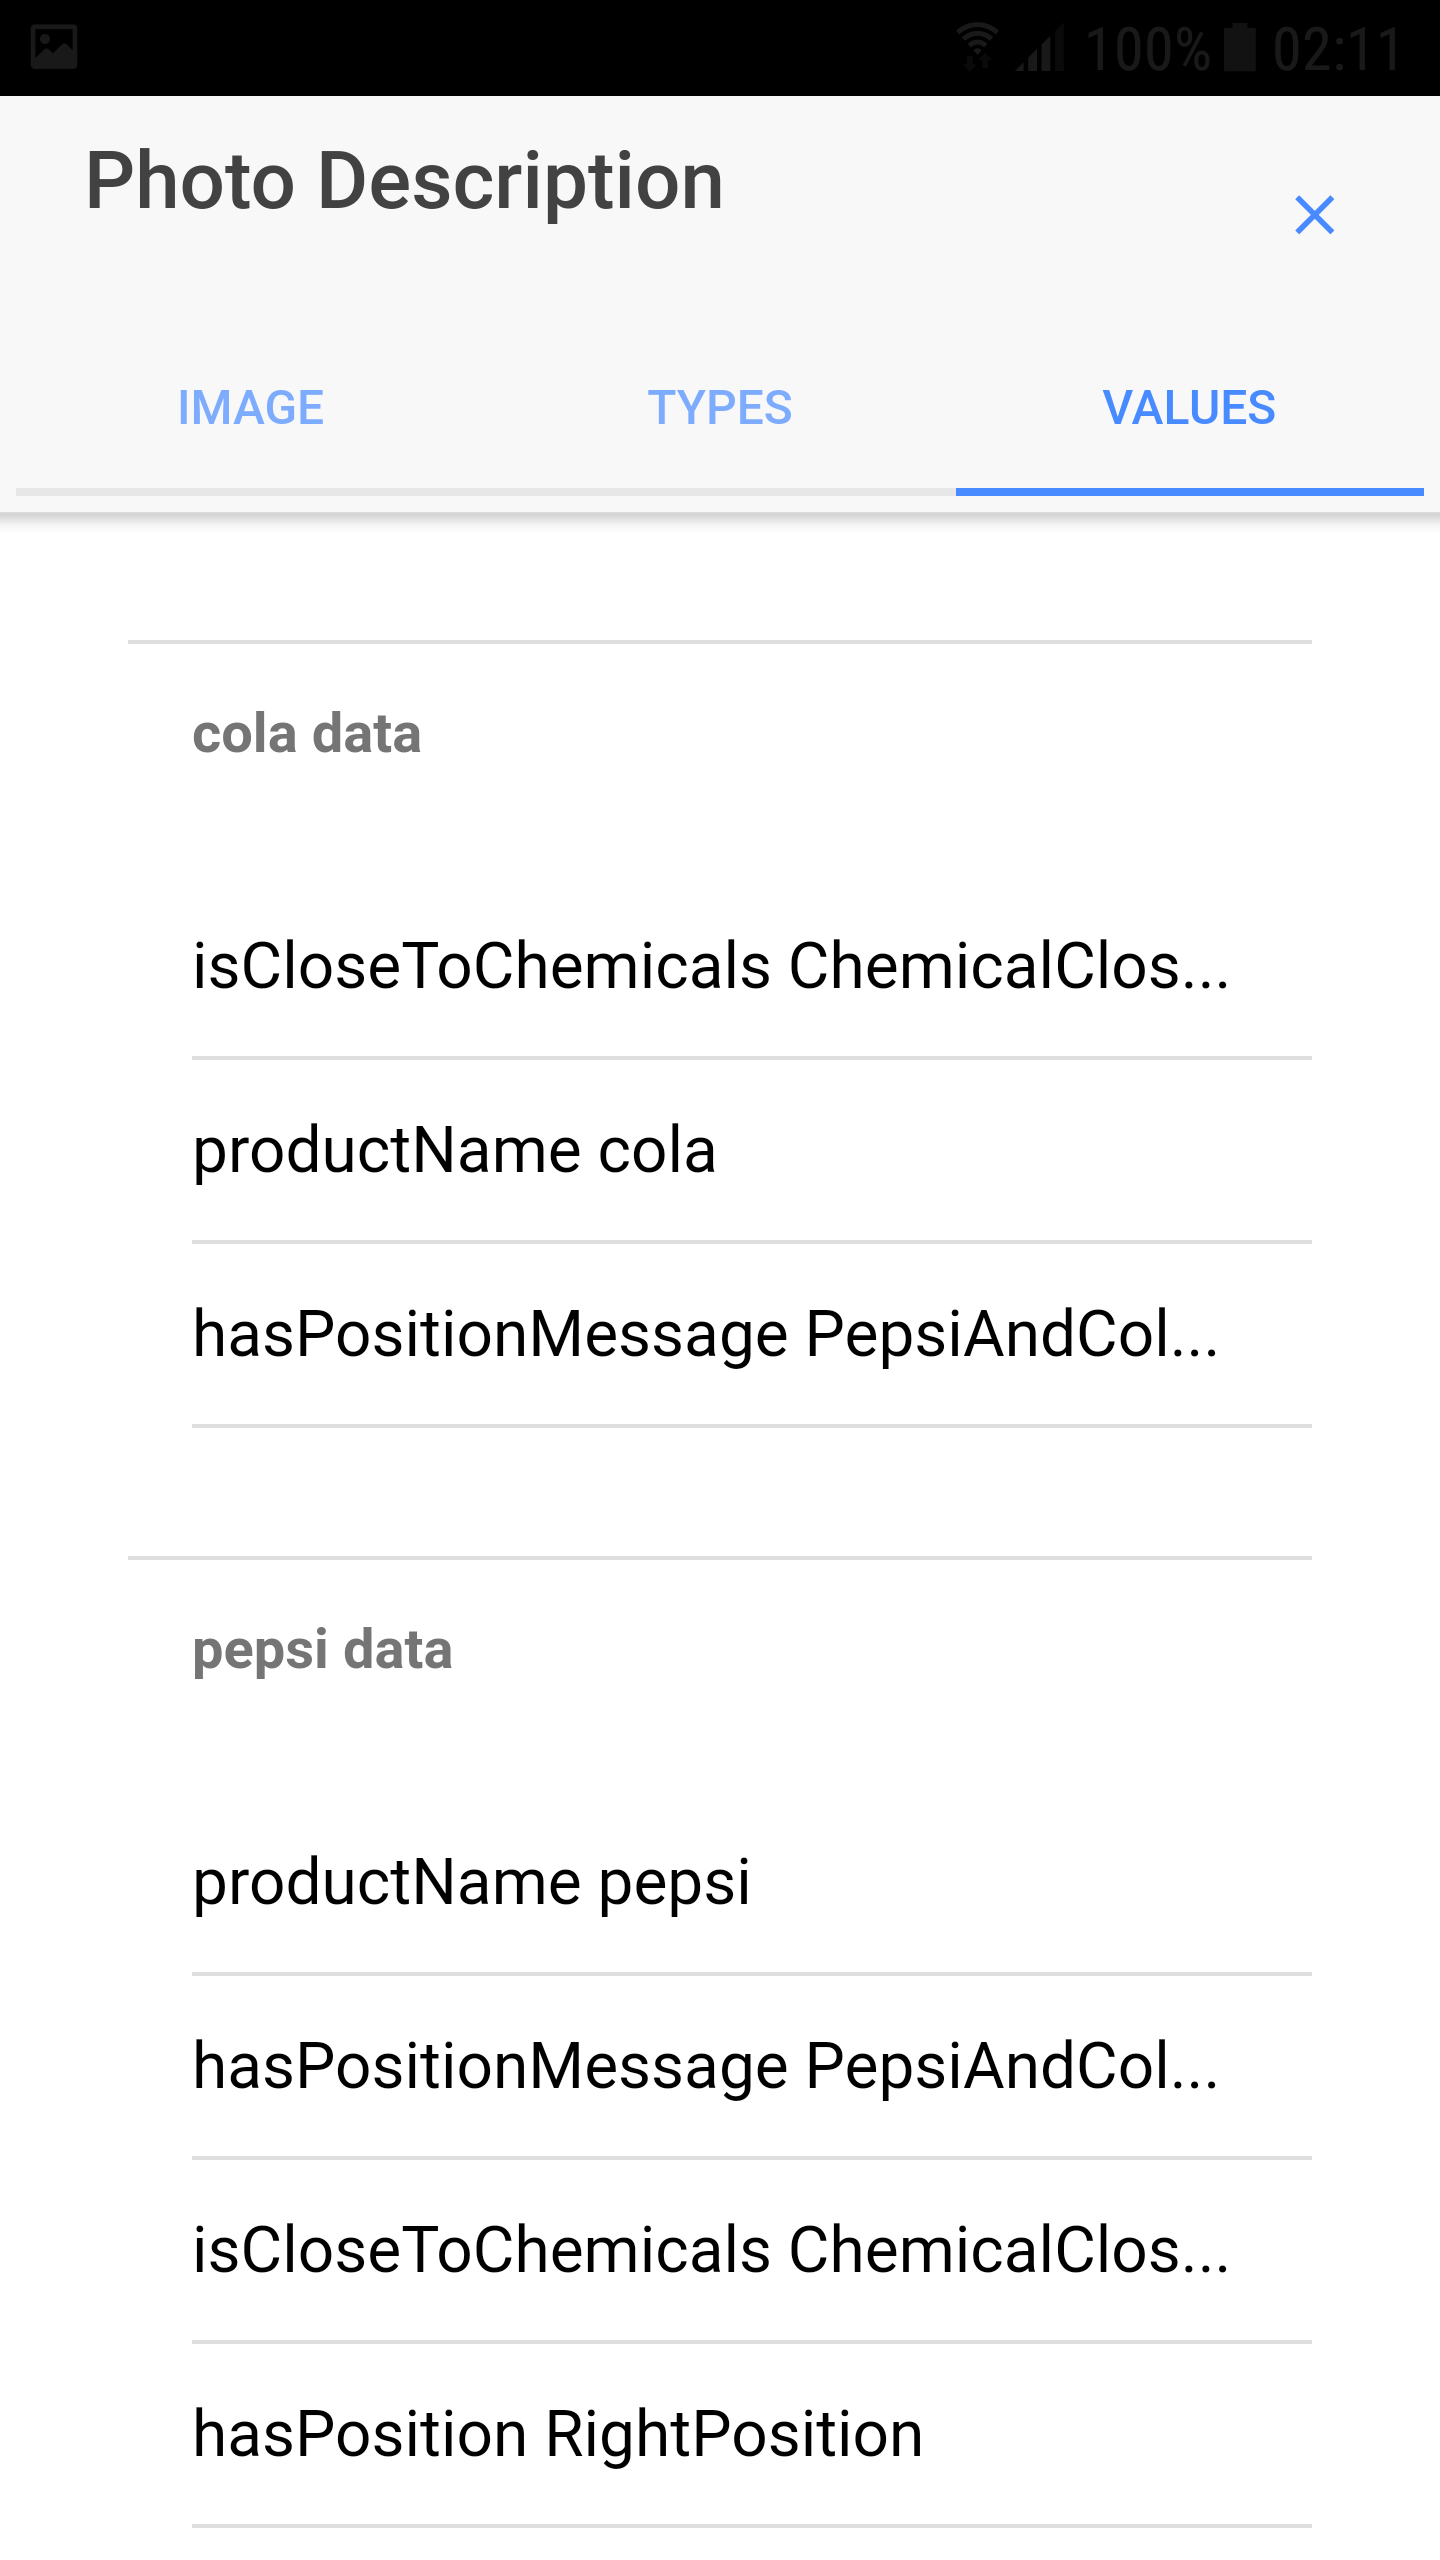
\includegraphics[width=0.4\textwidth]{images/values}}
	\quad
	\subfloat[Relacje pomiędzy indywiduami - wnioski.]{\label{odnosnik}
		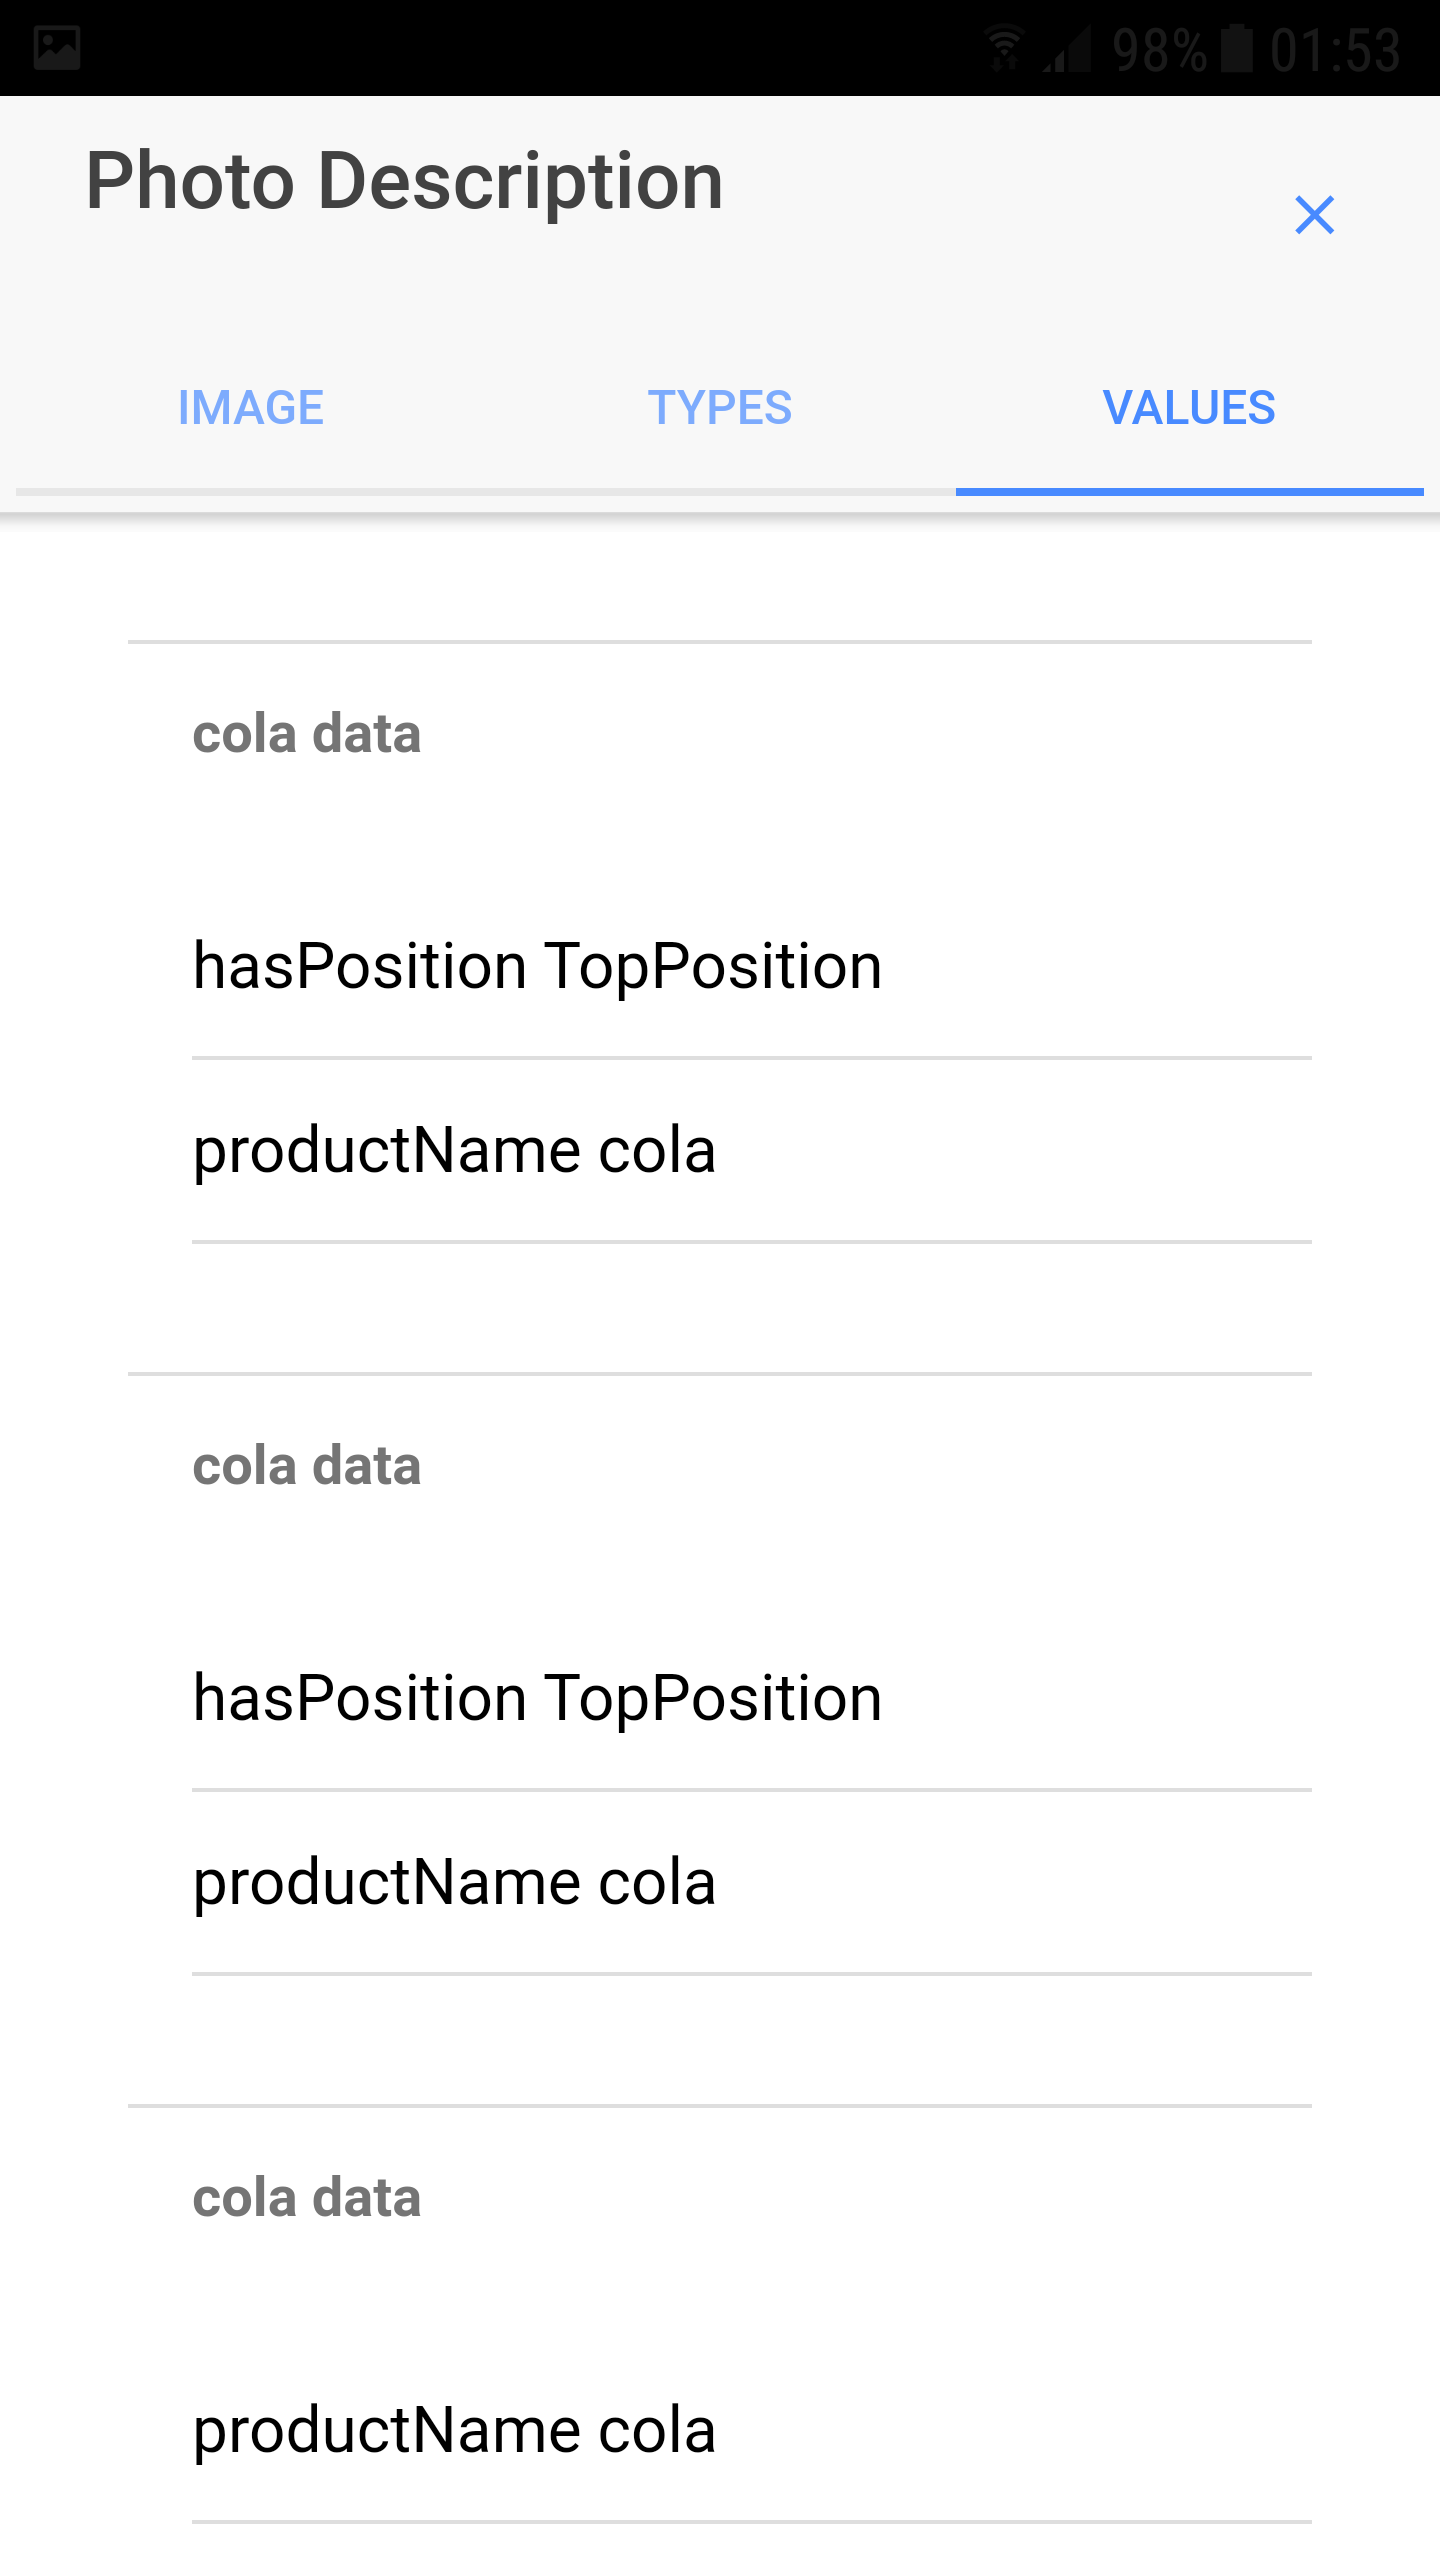
\includegraphics[width=0.4\textwidth]{images/values2}}
	\caption{Ekran szczegółów analizowanego zdjęcia - podzakładka wartości produktów.}
	\label{fig:details}
\end{figure}
}

\section{Historia}{
Użytkownik może wrócić do wcześniej wykonanych zdjęć oraz ich wyników. W tym celu z menu głównego należy wybrać pole archiwum (History). Wybranie zakładki spowoduje wyświetlenie zbioru przesłanych zdjęć wraz z wynikami przetwarzania. Na samym dole widoku znajduje się menu zbioru zdjęć historycznych. Nawigację można wykorzystać do przejścia do kolejnej strony wyników, cofnięcia się lub odświeżenia danych. Na każdym ze zdjęć można dokonać operacji usunięcia poprzez kliknięcie przycisku "Remove" oraz otrzymać szczegóły zdjęcia poprzez wybranie "Check details". Ekran szczegółów analizy nie różni się od ekranu otrzymanego zaraz po przesłaniu zdjęcia na serwer. Rysunek \ref{fig:historyAndReport} w punkcie a) przedstawia omawiany widok historii zdjęć.
}
\section{Raporty}{
Użytkownik z menu głównego może wybrać zakładkę "Raporty". Zostały w niej przedstawione statystyki indywidułów znajdujących się ontologii na produktu. Ponadto przedstawiają one podział nieprawidłowo ułożonych przedmiotów,  względem wszystkich dostępnych produktów. Raporty generowane są wraz z uruchomieniem aplikacji. Dzięki temu użytkownik każdorazowo logując się ma do dyspozycji aktualne dane.  Rysunek \ref{fig:historyAndReport} w punkcie b) przedstawia omawiany widok raportów i przedstawia kolejno - podział produktów niepoprawnie ułożonych względem wszystkich dostępnych przedmiotów oraz podział wywnioskowanych indywidułów.
}
\begin{figure}[h]
 	\centering
 	\subfloat[Historia Zdjęć.]{\label{odnosnik}
 		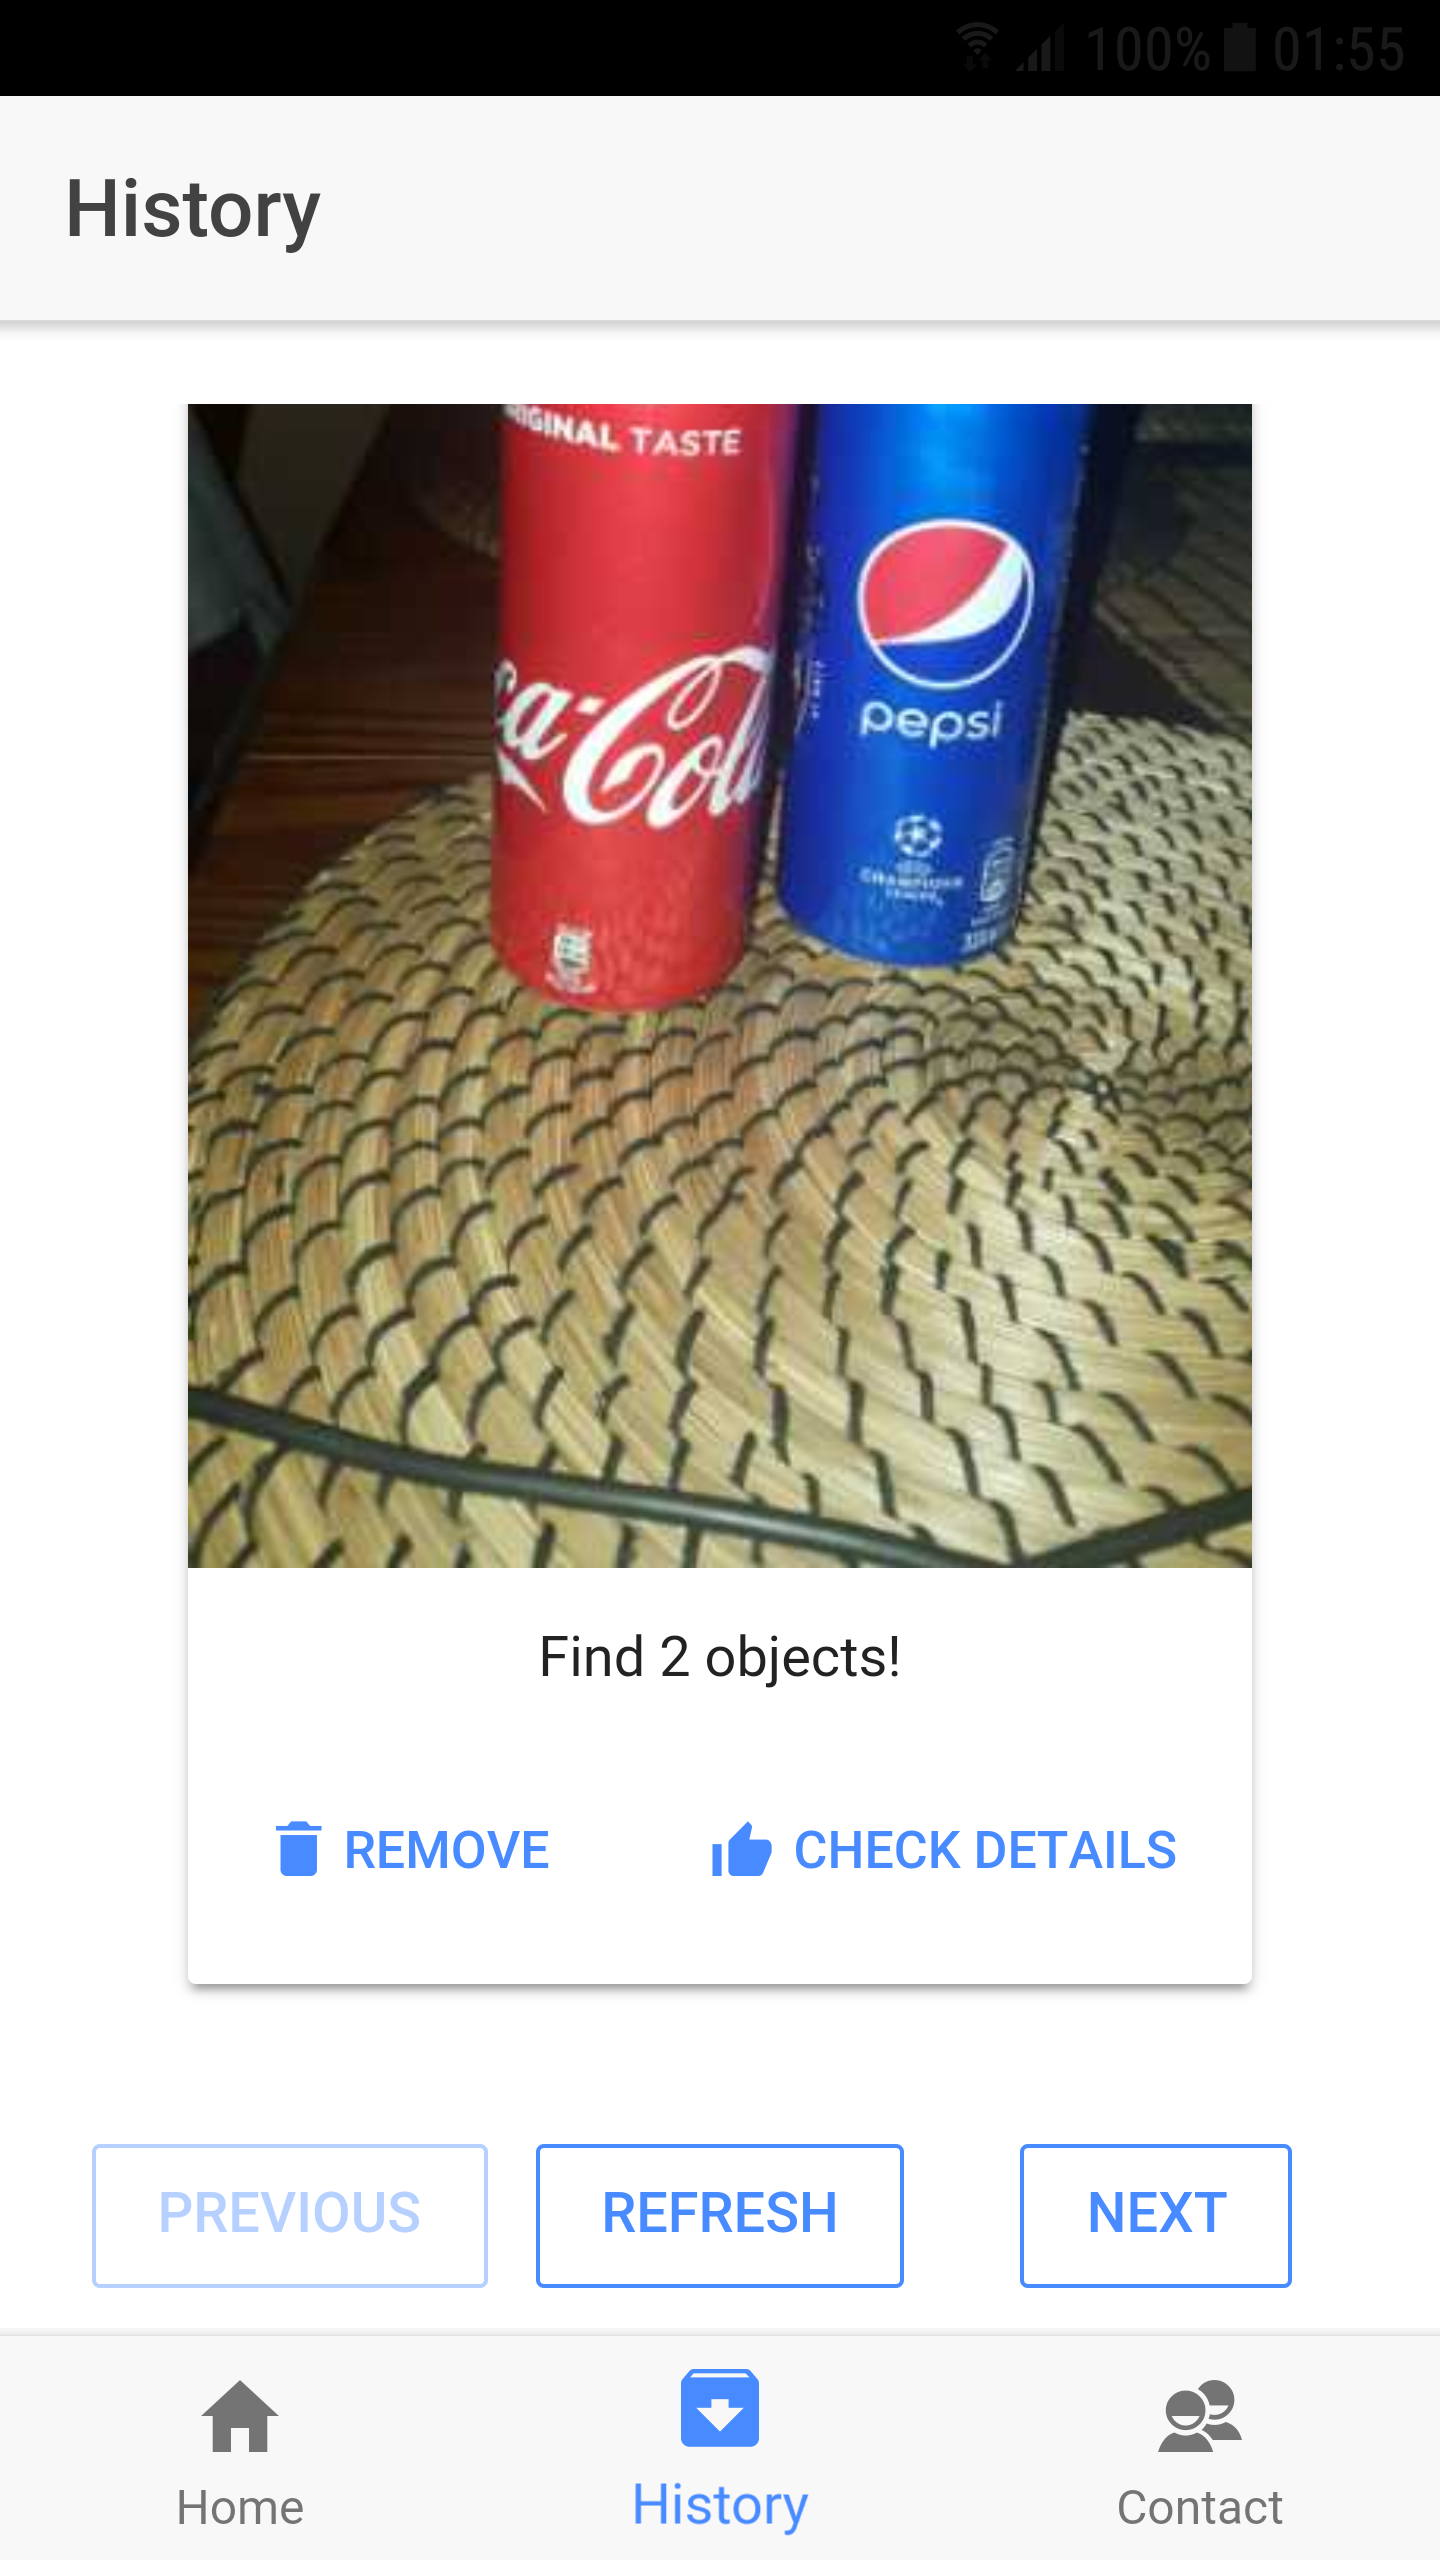
\includegraphics[width=0.4\textwidth]{images/history list}}
 	\quad
 	\subfloat[Raporty indywiduów ontologii.]{\label{odnosnik}
 		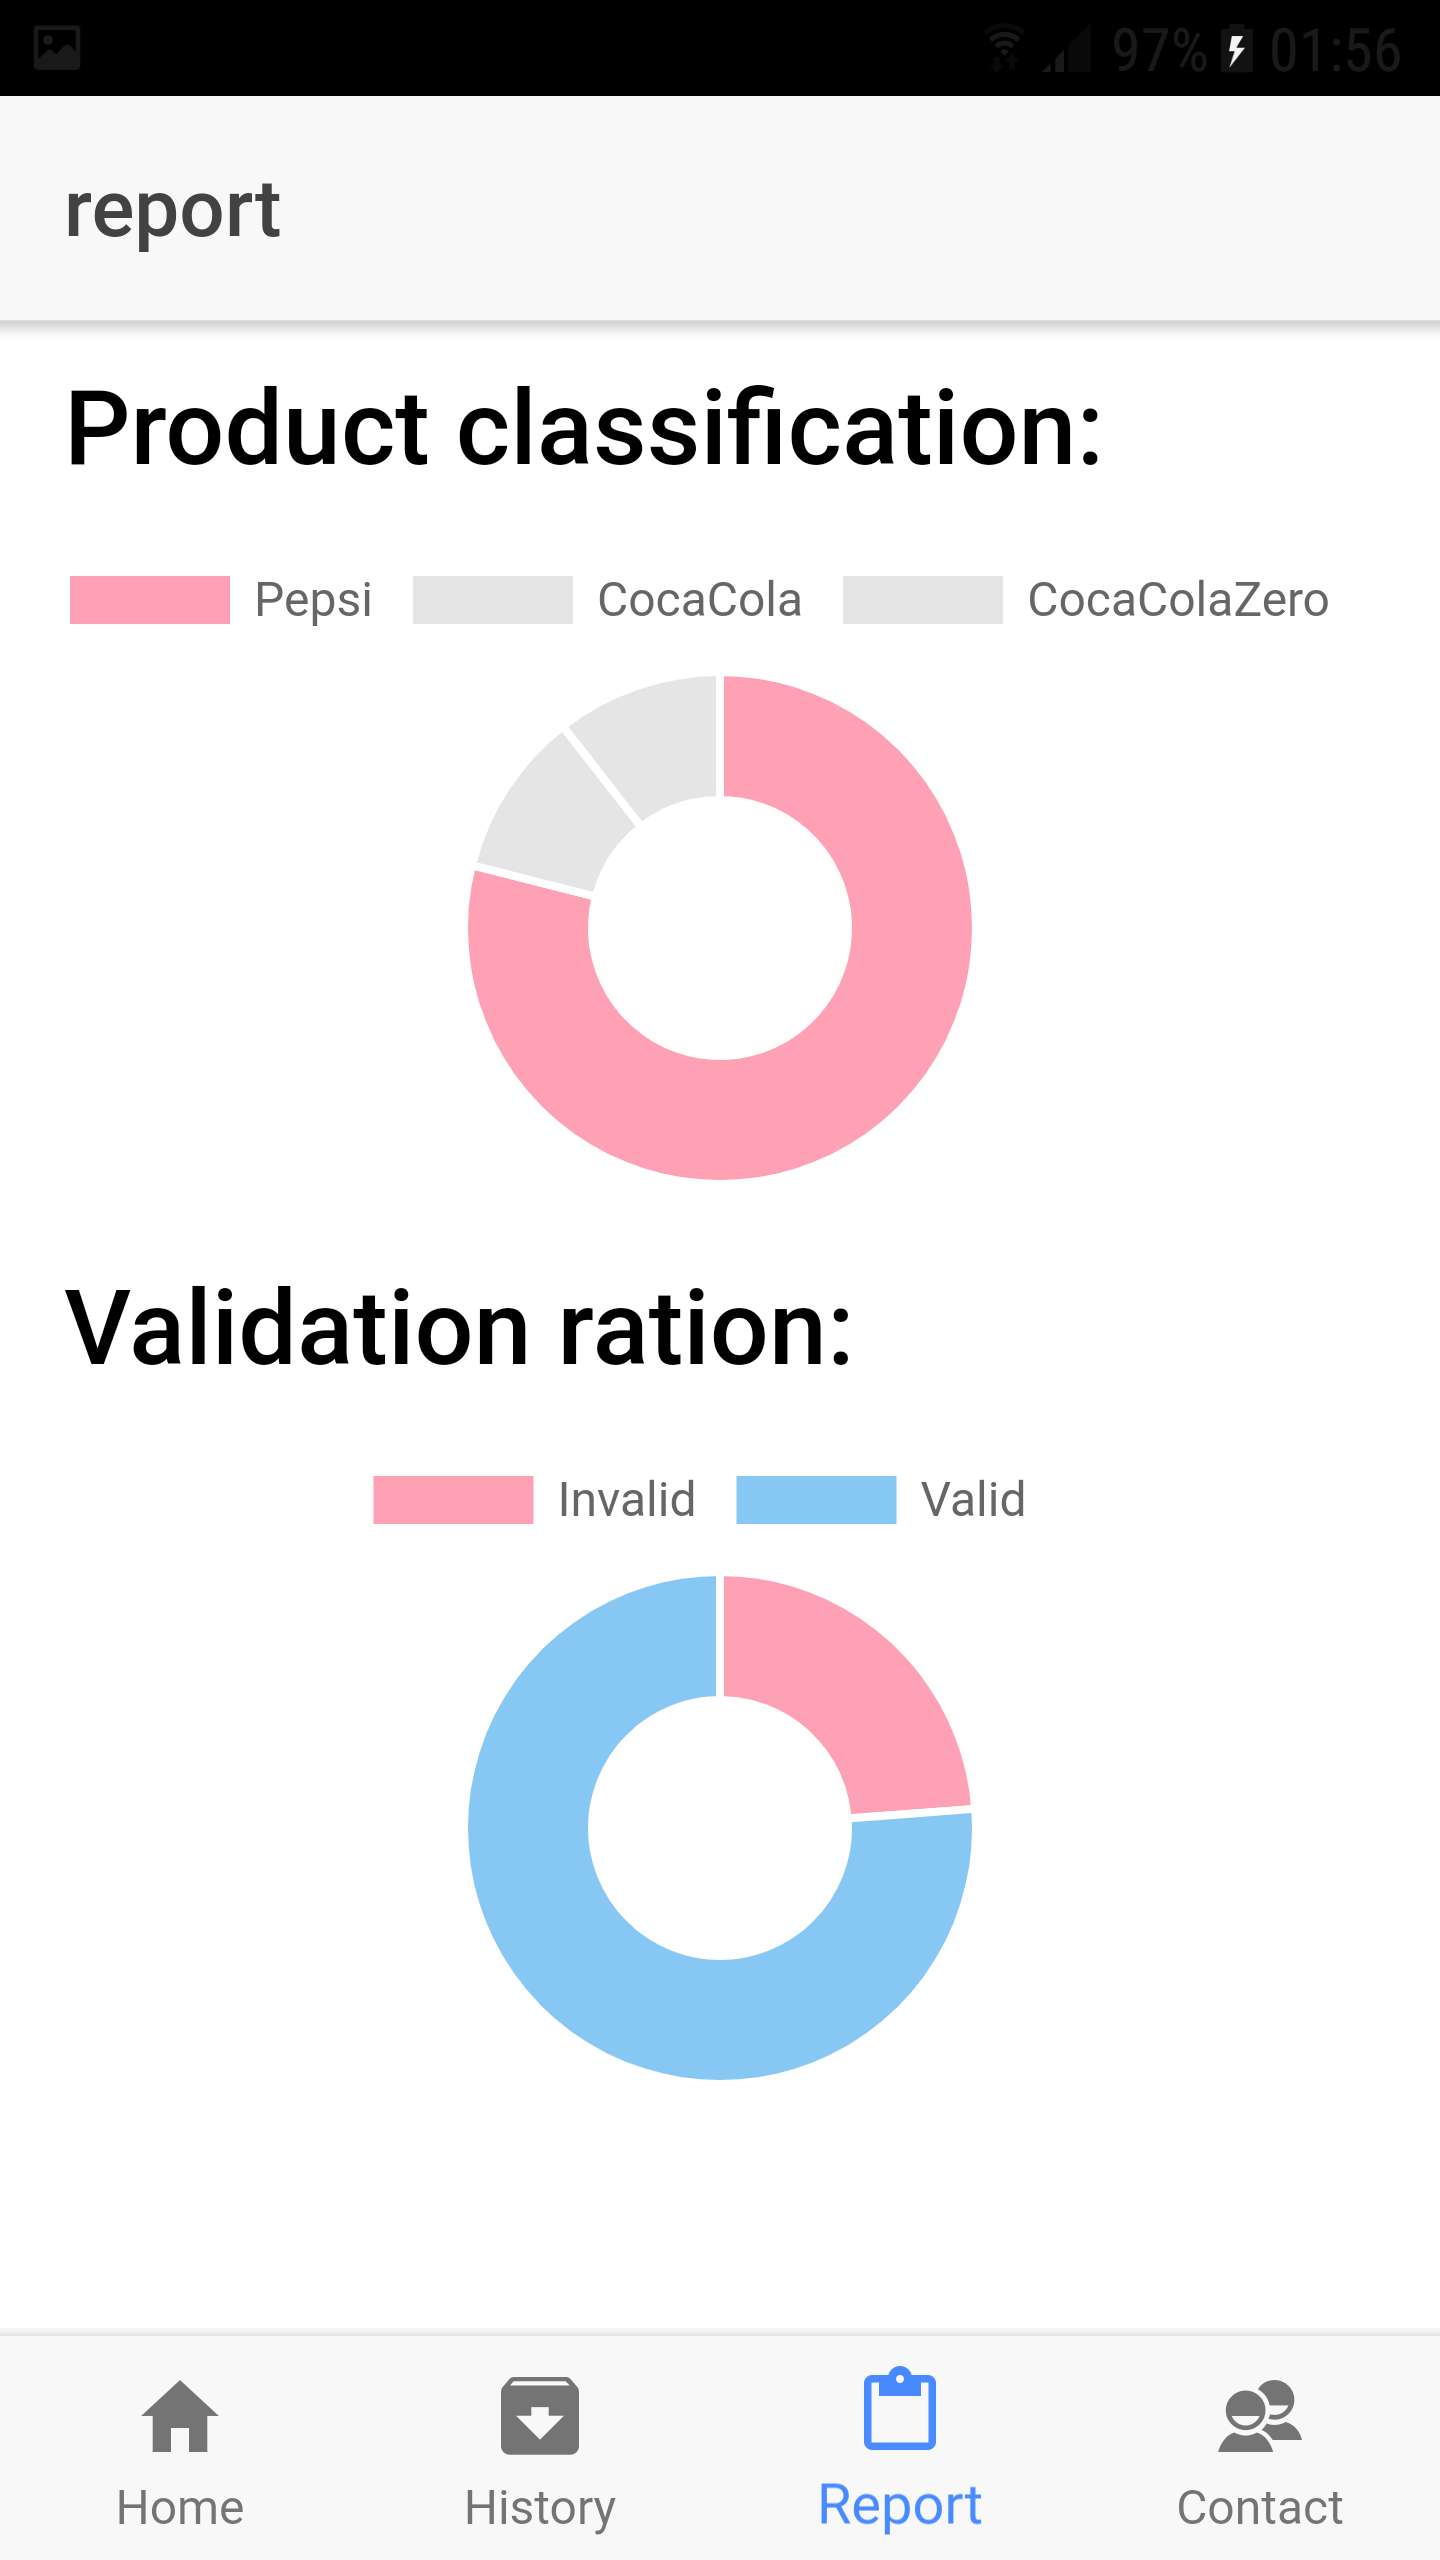
\includegraphics[width=0.4\textwidth]{images/reports}}
 	\caption{Ekran historii oraz raportów.}
	\label{fig:historyAndReport}
 \end{figure}

}




